\documentclass[10pt,aspectratio=169]{beamer}

\usepackage[T2A]{fontenc}
\usepackage[utf8]{inputenc}
\usepackage[russian]{babel}
\usepackage{graphicx}
\usepackage{booktabs}
\usepackage{array}
\usepackage{amsmath,amssymb}
\usepackage{tikz}
\usetikzlibrary{shapes.geometric,arrows.meta,positioning,fit,calc}
\usepackage{xcolor}

%% Navy blue corporate theme
\definecolor{navy}{RGB}{20,40,90}
\definecolor{accent}{RGB}{205,40,40}
\definecolor{soft}{RGB}{235,238,245}
\definecolor{good}{RGB}{30,120,60}

\usetheme{default}
\useoutertheme{infolines}
\useinnertheme{rectangles}
\setbeamercolor{frametitle}{bg=navy,fg=white}
\setbeamercolor{title}{fg=navy}
\setbeamercolor{structure}{fg=navy}
\setbeamercolor{footline}{fg=white,bg=navy}
\setbeamerfont{footline}{size=\tiny}
\setbeamertemplate{navigation symbols}{}
\setbeamertemplate{frametitle}
{\nointerlineskip%
  \begin{beamercolorbox}[wd=\paperwidth,ht=2.4ex,dp=1ex,leftskip=0.3cm]{frametitle}%
  \strut\insertframetitle\strut\end{beamercolorbox}}
\setbeamertemplate{footline}{%
  \leavevmode%
  \hbox{\begin{beamercolorbox}[wd=\paperwidth,ht=2.2ex,dp=1ex,leftskip=0.3cm,rightskip=0.3cm]{footline}%
    \tiny Р.Н.~Анаэдевха~~--~~Защита диссертации~~--~~НИЯУ МИФИ 2026 \hfill \insertframenumber/\inserttotalframenumber%
  \end{beamercolorbox}}%
}

\newcommand{\hl}[1]{\textcolor{accent}{\textbf{#1}}}
\newcommand{\bn}[1]{\textcolor{navy}{\textbf{#1}}}
\newcommand{\gd}[1]{\textcolor{good}{\textbf{#1}}}

\title{Состязательно-устойчивые модели и алгоритмы повышения
робастности и эффективности гибридных систем обнаружения и
предотвращения вторжений в распределённых и нестационарных
условиях}
\author{Аспирант: Роджер Ник Анаэдевха (А23--501)\\
Научный руководитель: Трофимов А.\,Г. (д.ф.-м.н., проф.)}
\institute{ИИКС, кафедра кибернетики № 22, НИЯУ МИФИ}
\date{Москва, 2026}

\begin{document}

% ============================================================
% Slide 1: Title
% ============================================================
{\setbeamertemplate{footline}{}
\begin{frame}[plain]
\begin{center}
\vspace{0.3cm}
{\small Национальный исследовательский ядерный университет <<МИФИ>>}\\[2pt]
{\small Институт интеллектуальных кибернетических систем (ИИКС),\\
кафедра кибернетики № 22}\\[12pt]
{\small Тема диссертации:}\\[6pt]
{\color{navy}\bfseries\large
<<Состязательно-устойчивые модели и алгоритмы\\
повышения робастности и эффективности\\
гибридных систем обнаружения и предотвращения вторжений\\
в распределённых и нестационарных условиях>>}\\[14pt]
\textbf{Аспирант:} Роджер Ник Анаэдевха (А23--501)\\
\textbf{Научный руководитель:} Трофимов Александр Геннадьевич
(к.т.н., д.т.н.)\\[8pt]
{\small Специальность 2.3.1 <<Системный анализ, управление
и обработка информации, статистика>>\\
(технические науки)}\\[14pt]
{\small Москва, 2026}
\end{center}
\end{frame}}

% ============================================================
% Slide 2: Тип рассматриваемых систем
% ============================================================
\begin{frame}{Тип рассматриваемых систем: гибридные системы
обнаружения и предотвращения вторжений (Hybrid IDPS)}
\vspace{-0.1cm}
\begin{columns}[T,onlytextwidth]
\column{0.55\textwidth}
\textbf{Hybrid IDPS} --- это \hl{ИИ/МО-усиленный} защитный
контур, объединяющий три канонических типа обнаружения:
\begin{itemize}
\item \bn{Сигнатурный} (Snort, Suricata, Zeek)
\item \bn{Поведенческий / аномалийный}
\item \bn{Анализ протоколов}
\end{itemize}
\medskip

\textbf{В отличие от коммерческих продуктов}
(Snort, Suricata, Zeek, Cisco~IPS, Palo~Alto, McAfee)~---
обучаемые компоненты встроены в защитный контур, а не
располагаются параллельно с ним.

\column{0.45\textwidth}
\begin{center}
\begin{tikzpicture}[scale=0.78,transform shape,
  every node/.style={font=\footnotesize}]
\node[draw=navy,rounded corners,fill=soft,minimum width=4.5cm,
  minimum height=0.6cm] (sig) {Сигнатурный детектор};
\node[draw=navy,rounded corners,fill=soft,minimum width=4.5cm,
  minimum height=0.6cm,below=0.2cm of sig] (beh) {Поведенческий детектор};
\node[draw=navy,rounded corners,fill=soft,minimum width=4.5cm,
  minimum height=0.6cm,below=0.2cm of beh] (prot) {Анализ протоколов};
\node[draw=accent,thick,rounded corners,fill=accent!10,
  minimum width=4.5cm,minimum height=1.0cm,below=0.3cm of prot,
  text width=4.2cm,align=center]
  (ai) {\textbf{Обучаемые компоненты\\(M1--M7, LLM)}};
\node[draw=navy,fill=navy,text=white,rounded corners,
  minimum width=4.5cm,minimum height=0.6cm,below=0.25cm of ai]
  (resp) {Политика реагирования $\pi$};
\draw[-{Stealth},navy] (sig.south)+(0,-0.05) -- ($(beh.north)+(0,0.05)$);
\draw[-{Stealth},navy] (beh.south)+(0,-0.05) -- ($(prot.north)+(0,0.05)$);
\draw[-{Stealth},accent] (prot.south)+(0,-0.05) -- ($(ai.north)+(0,0.05)$);
\draw[-{Stealth},navy] (ai.south)+(0,-0.05) -- ($(resp.north)+(0,0.05)$);
\end{tikzpicture}\\
{\scriptsize Многоуровневая архитектура Hybrid IDPS}
\end{center}
\end{columns}
\end{frame}

% ============================================================
% Slide 3: Актуальность темы исследования
% ============================================================
\begin{frame}{Актуальность темы исследования}
\begin{columns}[T,onlytextwidth]
\column{0.50\textwidth}
\textbf{Почему это исследование актуально:}
\begin{itemize}
\item Hybrid IDPS внедряются в \hl{критически важные системы}:
здравоохранение, финансы, промышленный IoT, автономные системы,
кибербезопасность
\item Их робастность \hl{отстаёт от точности на 25--65~п.\,п.}
в условиях атак
\item Hybrid IDPS объединяет \bn{сигнатурный, поведенческий и
протокольный} анализ~--- возмущение любого компонента
ставит под удар весь контур
\end{itemize}
\smallskip
\textbf{Задокументированные отказы Hybrid IDPS:}
\begin{itemize}
\item Здравоохранение: падение AUC до 25\%
\item Финансы: 25,7\%~$\to$~68,6\% ошибок
\item Промышленность: 94,2\%~$\to$~30\% коллапс
\item Кибербезопасность: $-$59\% обнаружения
\end{itemize}

\column{0.50\textwidth}
\textbf{Три сходящихся тренда:}\smallskip

\textbf{1. Масштаб.} Глобальный ущерб от кибератак достигает
\$10,5~трлн в год к 2025~г.; ИИ-инструменты SOC необходимы,
но уязвимы.\smallskip

\textbf{2. Регулирование.} NIST~AI~RMF, EU~AI~Act и сроки
перехода на PQC требуют \hl{сертифицированной} устойчивости,
а не только эмпирического тестирования.\smallskip

\textbf{3. Теоретический пробел.} Нет единой математической
основы, одновременно обеспечивающей устойчивость, приватность,
эффективность и точность Hybrid IDPS на динамических графовых
структурах.\smallskip

\begin{block}{}
\small\textbf{Данная диссертация} восполняет этот пробел:
единое описание Hybrid IDPS и 7~моделей с формальными
гарантиями по~3~условиям и~4~требованиям.
\end{block}
\end{columns}
\end{frame}

% ============================================================
% Slide 4: Области применения Hybrid IDPS и их текущие проблемы
% ============================================================
\begin{frame}{Области применения Hybrid IDPS и их текущие проблемы}
\textit{\small Hybrid IDPS развёрнуты в широком спектре
критически важных секторов, но во всех страдают от одних и тех
же недостатков.}
\vspace{0.1cm}
\begin{columns}[T,onlytextwidth]
\column{0.48\textwidth}
\textbf{Hybrid IDPS применяются в:}
\begin{itemize}
\item \bn{Здравоохранение}~--- защита электронных историй
болезни и медицинских устройств
\item \bn{Финансы}~--- защита от мошенничества с
транзакциями и отмывания денег
\item \bn{Кибербезопасность}~--- защита сетевого трафика,
графы сетевых устройств
\item \bn{Промышленность}~--- защита SCADA/АСУ ТП и
промышленных шлюзов
\item \bn{Автономные системы}~--- защита бортовых систем БПЛА
\item \bn{Облачные и микросервисные среды}
\end{itemize}

\column{0.48\textwidth}
\textbf{Их 4 критических недостатка:}
\begin{enumerate}
\item Запаздывание сигнатур на \hl{30--90~дней} относительно
новых угроз
\item Не могут адаптироваться к дрейфу без полного
переобучения
\item Слишком медленны на больших темпоральных
графах ($\mathcal{O}(P\cdot S)$ протокольный анализ)
\item Не могут обмениваться знаниями между организациями
без утечки данных
\end{enumerate}
\smallskip
\begin{block}{}
\small\textbf{Вывод:} требуется единое математическое описание
Hybrid IDPS, на основе которого строится семейство моделей,
устраняющих все четыре недостатка одновременно.
\end{block}
\end{columns}
\end{frame}

% ============================================================
% Slide 5: Степень разработанности темы
% ============================================================
\begin{frame}{Степень разработанности темы}
\begin{columns}[T,onlytextwidth]
\column{0.48\textwidth}
\textbf{Значительный вклад предшественников:}\smallskip\\
\textbf{IDPS и сетевая безопасность:}\\
А.\,А.~Бурлаков, А.\,С.~Марков, В.\,В.~Сачков; M.~Roesch
(Snort), V.~Paxson (Bro/Zeek)\medskip\\
\textbf{Графовое глубокое обучение:}\\
T.\,N.~Kipf, M.~Welling (GCN); P.~Veli\v{c}kovi\'{c} (GAT);
W.\,L.~Hamilton (GraphSAGE); X.~Xu (GIN)\medskip\\
\textbf{Нейронные ОДУ / СДУ:}\\
R.\,T.\,Q.~Chen (Neural ODE); Rubanova (латентные ОДУ);
Kidger (нейронные КДУ)\medskip\\
\textbf{Состязательное МО:}\\
A.~Madry (PGD); N.~Carlini, D.~Wagner (C\&W); J.~Cohen
(рандомизированное сглаживание)

\column{0.48\textwidth}
\textbf{Федеративное обучение / приватность:}\\
B.~McMahan (FedAvg); P.~Blanchard (византийский SGD);
K.~Bonawitz; H.~McMahan (DP)\medskip\\
\textbf{Модели пространств состояний:}\\
A.~Gu, T.~Dao (S4, Mamba); Smith~(S5); Behrouz (Graph Mamba)\medskip

\begin{alertblock}{Что остаётся нерешённым}
\small Ни одна из существующих работ не обеспечивает
одновременного выполнения для Hybrid IDPS:
\begin{enumerate}
\item Сертифицированной динамики непрерывного времени
\item Византийско-устойчивой федерации с ДП
\item $\mathcal{O}(L\log L)$ вывода с дистилляцией
\item Калиброванной декомпозиции неопределённости
\item Теоретико-игровой сертификации без сожаления
\end{enumerate}
\end{alertblock}
\end{columns}
\end{frame}

% ============================================================
% Slide 6: Почему важна робастность Hybrid IDPS?
% ============================================================
\begin{frame}{Почему важна робастность Hybrid IDPS?}
\begin{columns}[T,onlytextwidth]
\column{0.55\textwidth}
Hybrid IDPS применяются в:
\begin{itemize}
\item \bn{Сетевой безопасности} (графы трафика)
\item \bn{Здравоохранении} (молекулярные / графы пациентов)
\item \bn{Финансах} (графы транзакций)
\item \bn{Автономных системах} (графы слияния датчиков БПЛА)
\end{itemize}
\smallskip
\textcolor{accent}{\textbf{Ключевая уязвимость:}}
обучаемые компоненты Hybrid IDPS принимают \hl{два входа}:
\begin{itemize}
\item Входные данные $X\in\mathbb{R}^{n\times d}$ (признаки)
\item Входную структуру $A\in\{0,1\}^{n\times n}$ (матрица
смежности)
\end{itemize}
Возмущение \emph{любого} из них нарушает выход~$\Rightarrow$
сертификат робастности должен покрывать оба входа.

\column{0.45\textwidth}
\begin{center}
\begin{tikzpicture}[scale=0.85,transform shape,
  every node/.style={font=\scriptsize}]
\node[draw=navy,fill=soft,rounded corners,minimum width=2.8cm,
  minimum height=0.7cm] (X) {Входные данные $X\in\mathbb{R}^{n\times d}$};
\node[draw=navy,fill=soft,rounded corners,minimum width=2.8cm,
  minimum height=0.7cm,below=0.4cm of X] (A) {Структура $A\in\{0,1\}^{n\times n}$};
\node[draw=accent,thick,fill=accent!10,rounded corners,
  minimum width=3.2cm,minimum height=1.0cm,right=1.2cm of X,
  yshift=-0.65cm,text width=3cm,align=center]
  (G) {Обучаемый компонент Hybrid IDPS ($f_\theta$)};
\node[draw=good,fill=good!10,rounded corners,minimum width=2.8cm,
  minimum height=0.7cm,right=1cm of G] (Z) {Представление $Z$};
\draw[-{Stealth},navy] (X.east) -- (G.west);
\draw[-{Stealth},navy] (A.east) -- (G.west);
\draw[-{Stealth},good] (G.east) -- (Z.west);
\end{tikzpicture}\\
{\scriptsize Двойственная природа входов: данные ($X$) и
структура ($A$) обрабатываются совместно}
\end{center}
\end{columns}
\end{frame}

% ============================================================
% Slide 7: Зачем непрерывное время
% ============================================================
\begin{frame}{Зачем переходить от дискретного к непрерывному времени в Hybrid IDPS?}
\begin{columns}[T,onlytextwidth]
\column{0.55\textwidth}
\textcolor{accent}{\textbf{Дискретные обучаемые компоненты
(уязвимы):}} фиксированный такт обновления $\to$ модель
\emph{пропускает} события между шагами, ошибка не ограничена.\smallskip

\textcolor{good}{\textbf{Непрерывно-временные компоненты
(робастны):}} гладкий поток состояний $\to$ фиксирует все
события, чувствительность ограничена константой Липшица.\smallskip

\textbf{Сертификат робастности.} Если $\|x_1-x_2\|\le\varepsilon$,
то $\|h_1(T)-h_2(T)\|\le e^{L_g T}\varepsilon$. Дискретные
обучаемые модули такого сертификата не обеспечивают.

\column{0.45\textwidth}
\begin{block}{Неравенство Гр\"енуолла}
\[
\|h_1(T)-h_2(T)\| \;\le\; e^{L_g T}\,\|x_1-x_2\|
\]
\end{block}
\smallskip
\textbf{Обозначения:}
\begin{itemize}\setlength\itemsep{0pt}
\item[$h_i(T)$] скрытое состояние траектории $i$ в момент $T$
\item[$x_i$] начальный вход (признаки + структура)
\item[$L_g$] константа Липшица векторного поля ОДУ
\item[$T$] горизонт интегрирования
\item[$e^{L_g T}$] максимальный коэффициент усиления
возмущения
\end{itemize}
\end{columns}
\end{frame}

% ============================================================
% Slide 8: Причины меньшей уязвимости
% ============================================================
\begin{frame}{Причины, по которым непрерывно-временные компоненты Hybrid IDPS менее уязвимы}
\vspace{0.5cm}
\begin{enumerate}
\item Представления узлов графа эволюционируют согласно
дифференциальному уравнению с \hl{ограниченной константой
Липшица}.
\smallskip
\item Малые возмущения входа могут вызвать лишь
\hl{ограниченные, гладкие изменения выхода}~--- управляющий
поток математически ограничивает степень изменения предсказания
противником.
\smallskip
\item Дискретные обучаемые модули Hybrid IDPS не имеют такого
непрерывного механизма~--- возмущения \hl{непредсказуемо
накапливаются} от слоя к слою и могут обходить сигнатурный
и поведенческий контуры.
\smallskip
\item Непрерывно-временная динамика естественно согласуется с
многомасштабными временными константами Hybrid IDPS:
$\tau_{\text{packet}}{=}1$\,c, $\tau_{\text{session}}{=}60$\,c,
$\tau_{\text{campaign}}{=}3600$\,c.
\end{enumerate}
\end{frame}

% ============================================================
% Slide 9: Задокументированные отказы Hybrid IDPS
% ============================================================
\begin{frame}{Почему это исследование критически важно: задокументированные отказы Hybrid IDPS}
\small
\begin{tabular}{p{2.0cm}p{4.0cm}p{3.7cm}p{2.8cm}}
\toprule
\textbf{Область} & \textbf{Что произошло} & \textbf{Последствия} & \textbf{Источник} \\
\midrule
Здравоохр.\ &
Атака на чувствительность рёбер GNN-IDPS для медицинских
изображений (Tox21, ClinTox, SIDER) &
$\sim$25\% падение AUC; токсичные потоки классифицированы
как безопасные &
Sci.\ Rep. 15, 2025\\
\midrule
Финансы &
MonTi-атака на встраивание ML-детекторов мошенничества в
банковский Hybrid IDPS (CARE-GNN, PC-GNN, GAGA) &
25,7\%~$\to$~68,6\% ошибок; мошеннические группы уклоняются от
обнаружения & AAAI 2025, arXiv:2412.18370 \\
\midrule
Промышл. &
Отравление данных в федеративных Hybrid IDPS промышленного
IoT (Edge-IIoTset, ne-IID) &
94,2\%~$\to$~30,0\% точности; коллапс на 64 узлах &
IEEE/arXiv, 2023 \\
\midrule
Кибербезоп.\ &
PROVNINJA обход GNN-компонентов IDPS обнаружения
(S-GAT, Prov-GAT) через подмену системных вызовов &
Обнаружение $-$59\%; APT-атаки становятся невидимыми &
USENIX Security 2023 \\
\bottomrule
\end{tabular}
\smallskip
\begin{alertblock}{}
\small\textbf{Вывод:} робастность Hybrid IDPS отстаёт от
точности на 25--65~п.\,п. во всех критически важных
областях. $\Rightarrow$ Этот разрыв мотивирует всю
диссертацию.
\end{alertblock}
\end{frame}

% ============================================================
% Slide 10: Зачем нужна распределённая среда
% ============================================================
\begin{frame}{Зачем нужна распределённая среда?}
\begin{columns}[T,onlytextwidth]
\column{0.50\textwidth}
Множество организаций владеют графовыми данными Hybrid IDPS
и \hl{не могут ими делиться}~--- больницы, банки, ЦОД.
Совместная модель должна обучаться через \bn{федеративное
обучение}~--- ни одна сторона не видит сырых данных другой.
\smallskip

\textbf{Почему это срочно:}
\begin{enumerate}\setlength\itemsep{0pt}
\item Злоумышленники обманывают обучаемые компоненты Hybrid IDPS
малыми возмущениями
\item Распределения смещаются после развёртывания
\item Законы о конфиденциальности ограничивают обмен данными
\item Периферийные устройства требуют вывода в реальном времени
\end{enumerate}
\smallskip
\textcolor{accent}{Ни один существующий подход не решает все
четыре проблемы одновременно.}

\column{0.50\textwidth}
\begin{center}
\begin{tikzpicture}[scale=0.78,transform shape,
  every node/.style={font=\scriptsize}]
\node[draw=navy,fill=navy,text=white,rounded corners,
  minimum width=3.0cm,minimum height=0.7cm] (g) {Глобальная модель};
\node[draw=navy,fill=soft,rounded corners,minimum width=1.6cm,
  minimum height=0.5cm,below=1.5cm of g,xshift=-2.5cm] (h)
  {Больница $G_1$};
\node[draw=navy,fill=soft,rounded corners,minimum width=1.6cm,
  minimum height=0.5cm,below=1.5cm of g] (b) {Банк $G_2$};
\node[draw=navy,fill=soft,rounded corners,minimum width=1.6cm,
  minimum height=0.5cm,below=1.5cm of g,xshift=2.5cm] (c)
  {ЦОД $G_3$};
\node[draw=accent,fill=accent!15,rounded corners,minimum width=1.6cm,
  minimum height=0.5cm,below=0.5cm of h] (a)
  {Византийский противник};
\draw[-{Stealth},navy] (h) -- (g) node[midway,left,font=\tiny]{$\nabla_1$};
\draw[-{Stealth},navy] (b) -- (g) node[midway,right,font=\tiny]{$\nabla_2$};
\draw[-{Stealth},navy] (c) -- (g) node[midway,right,font=\tiny]{$\nabla_3$};
\draw[-{Stealth},accent,dashed] (a) -- (g);
\node[above=0cm of g,font=\scriptsize] {ОТ выравн.~|~ДП $\varepsilon{=}0{,}85$};
\end{tikzpicture}\\[2pt]
{\scriptsize Каждая организация хранит данные локально~---
передаются только градиенты $\to$ робастная агрегация}\\[4pt]
\textbf{3 гарантии:} византийская устойчивость + дифф.
приватность + ОТ-выравнивание
\end{center}
\end{columns}
\end{frame}

% ============================================================
% Slide 11: Развёртывание в реальном сценарии
% ============================================================
\begin{frame}{Развёртывание в реальном сценарии}
\begin{columns}[T,onlytextwidth]
\column{0.50\textwidth}
\textbf{Проблема:} После развёртывания Hybrid IDPS реальные
данные графа \hl{дрейфуют}:
\begin{itemize}
\item Топологии эволюционируют
\item Паттерны атак меняются
\item Появляются новые протоколы
\end{itemize}
\smallskip
Статические Hybrid IDPS \emph{незаметно} теряют точность
без предупреждения~--- устаревшая модель опасна. \textbf{Решение:}
встроить в Hybrid IDPS обучаемые компоненты, которые:
\begin{itemize}
\item Обнаруживают сдвиг распределения онлайн
\item Адаптируются без забывания (без полного переобучения)
\item Количественно оценивают неопределённость для маркировки
новых входов
\end{itemize}

\column{0.50\textwidth}
\begin{center}
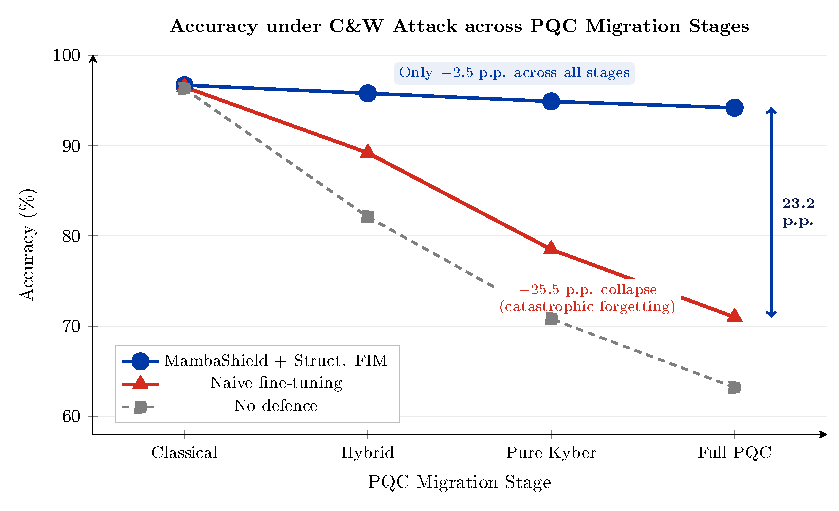
\includegraphics[width=\linewidth]{figures/fig_pqc_migration_robustness.pdf}\\[2pt]
{\scriptsize Зоны: обучение $\to$ дрейф $\to$ адаптация.
Статическая модель проседает; адаптивная сохраняет точность
за счёт байесовского апост.~+ сублинейного регрета
$\mathcal{O}(\sqrt{T\log|S|})$ + калибровки ECE}
\end{center}
\end{columns}
\end{frame}

% ============================================================
% Slide 12: Проблема эффективности
% ============================================================
\begin{frame}{Проблема эффективности}
Существующие архитектуры обучаемых компонентов Hybrid IDPS,
включая модели на основе трансформеров, масштабируются
\hl{квадратично} ($\mathcal{O}(L^2)$) с длиной
последовательности~--- каждый узел должен обращать внимание
на каждый другой узел, что делает их слишком медленными и
ресурсоёмкими для вывода в реальном времени на больших
темпоральных графах с миллионами событий.
\medskip

\begin{center}
\begin{tikzpicture}[every node/.style={font=\small}]
\node[draw=navy,fill=soft,rounded corners,minimum width=3cm,
  minimum height=1cm] (t) {Трансформер\\$\mathcal{O}(L^2)$};
\node[draw=good,fill=good!10,rounded corners,minimum width=3cm,
  minimum height=1cm,right=2cm of t] (s) {SSM (MambaShield)\\$\mathcal{O}(L\log L)$};
\draw[-{Stealth},accent,thick] (t) -- (s);
\end{tikzpicture}
\end{center}
\medskip

Литература показывает, что \bn{модели пространства состояний
(SSM)} более эффективны, снижая стоимость до
$\mathcal{O}(L\log L)$ за счёт БПФ-свёрток и обеспечивая
развёртывание на периферийных устройствах, где модели
масштаба трансформеров неприменимы.
\smallskip

\begin{alertblock}{}
\small Поэтому в Hybrid IDPS предложено перенести фокус с
трансформеров на SSM (MambaShield, M4) и сохранить
трансформер только для уточнения неопределённости (M5).
\end{alertblock}
\end{frame}

% ============================================================
% Slide 13: Поэтапный охват работы
% ============================================================
\begin{frame}{Поэтапный охват работы}
\begin{center}
\begin{tikzpicture}[every node/.style={font=\footnotesize}]
\node[draw=navy,fill=soft,rounded corners,minimum width=2.6cm,
  minimum height=1.2cm,text width=2.4cm,align=center]
  (a) {Перейти на НВ от ДВ\\(дин.\ графы эволюц.)};
\node[draw=navy,fill=soft,rounded corners,minimum width=2.6cm,
  minimum height=1.2cm,text width=2.4cm,align=center,right=0.5cm of a]
  (b) {Обеспечить обучение в распред.\ среде};
\node[draw=navy,fill=soft,rounded corners,minimum width=2.6cm,
  minimum height=1.2cm,text width=2.4cm,align=center,right=0.5cm of b]
  (c) {Повысить эффективность для больших графов};
\node[draw=navy,fill=soft,rounded corners,minimum width=2.6cm,
  minimum height=1.2cm,text width=2.4cm,align=center,right=0.5cm of c]
  (d) {Адаптироваться к нестац.\ условиям};
\draw[-{Stealth},navy,thick] (a) -- (b) node[midway,above,font=\tiny]{основа};
\draw[-{Stealth},navy,thick] (b) -- (c) node[midway,above,font=\tiny]{развёртыв.};
\draw[-{Stealth},navy,thick] (c) -- (d) node[midway,above,font=\tiny]{эффективн.};
\draw[-{Stealth},accent,dashed] (d.south) to[bend left=40] node[midway,below,font=\tiny]{обратная связь} (a.south);
\end{tikzpicture}
\end{center}
\medskip
Они образуют \hl{логическую цепочку} в построении Hybrid IDPS:
выход каждой задачи является входом для следующей.
\smallskip

\textcolor{accent}{Ни один существующий подход не решает все
четыре задачи одновременно при 3~условиях $\times$~4~требованиях
Hybrid IDPS.}
\end{frame}

% ============================================================
% Slide 14: Пространство задач Hybrid IDPS
% ============================================================
\begin{frame}{Пространство задач Hybrid IDPS: условия и требования}
\begin{columns}[T,onlytextwidth]
\column{0.50\textwidth}
\textbf{Три рабочих условия (P-условия):}
\begin{itemize}
\item У1. Состязательная среда (P1)
\item У2. Распределённая среда (P4)
\item У3. Нестационарность (P6)
\end{itemize}
\smallskip
\textbf{Доп.\ свойство:} человеческий фактор~--- триаж
аналитика (P5).

\column{0.50\textwidth}
\textbf{Четыре сквозных требования (T):}
\begin{itemize}
\item Т1. Робастность (P2)
\item Т2. Точность
\item Т3. Эффективность (P3)
\item Т4. Дифференциальная приватность
\end{itemize}
\end{columns}
\medskip
\begin{block}{}
\small Эти три рабочих условия и четыре сквозных требования
независимы~--- они определяют пространство, в котором любая
обучаемая компонента Hybrid IDPS должна функционировать
надёжно. В диссертации предложены модели M1--M7, удовлетворяющие
всем 12~пересечениям одновременно.
\end{block}
\end{frame}

% ============================================================
% Slide 15: Общая фреймворк
% ============================================================
\begin{frame}{Общая фреймворк работы}
\begin{center}
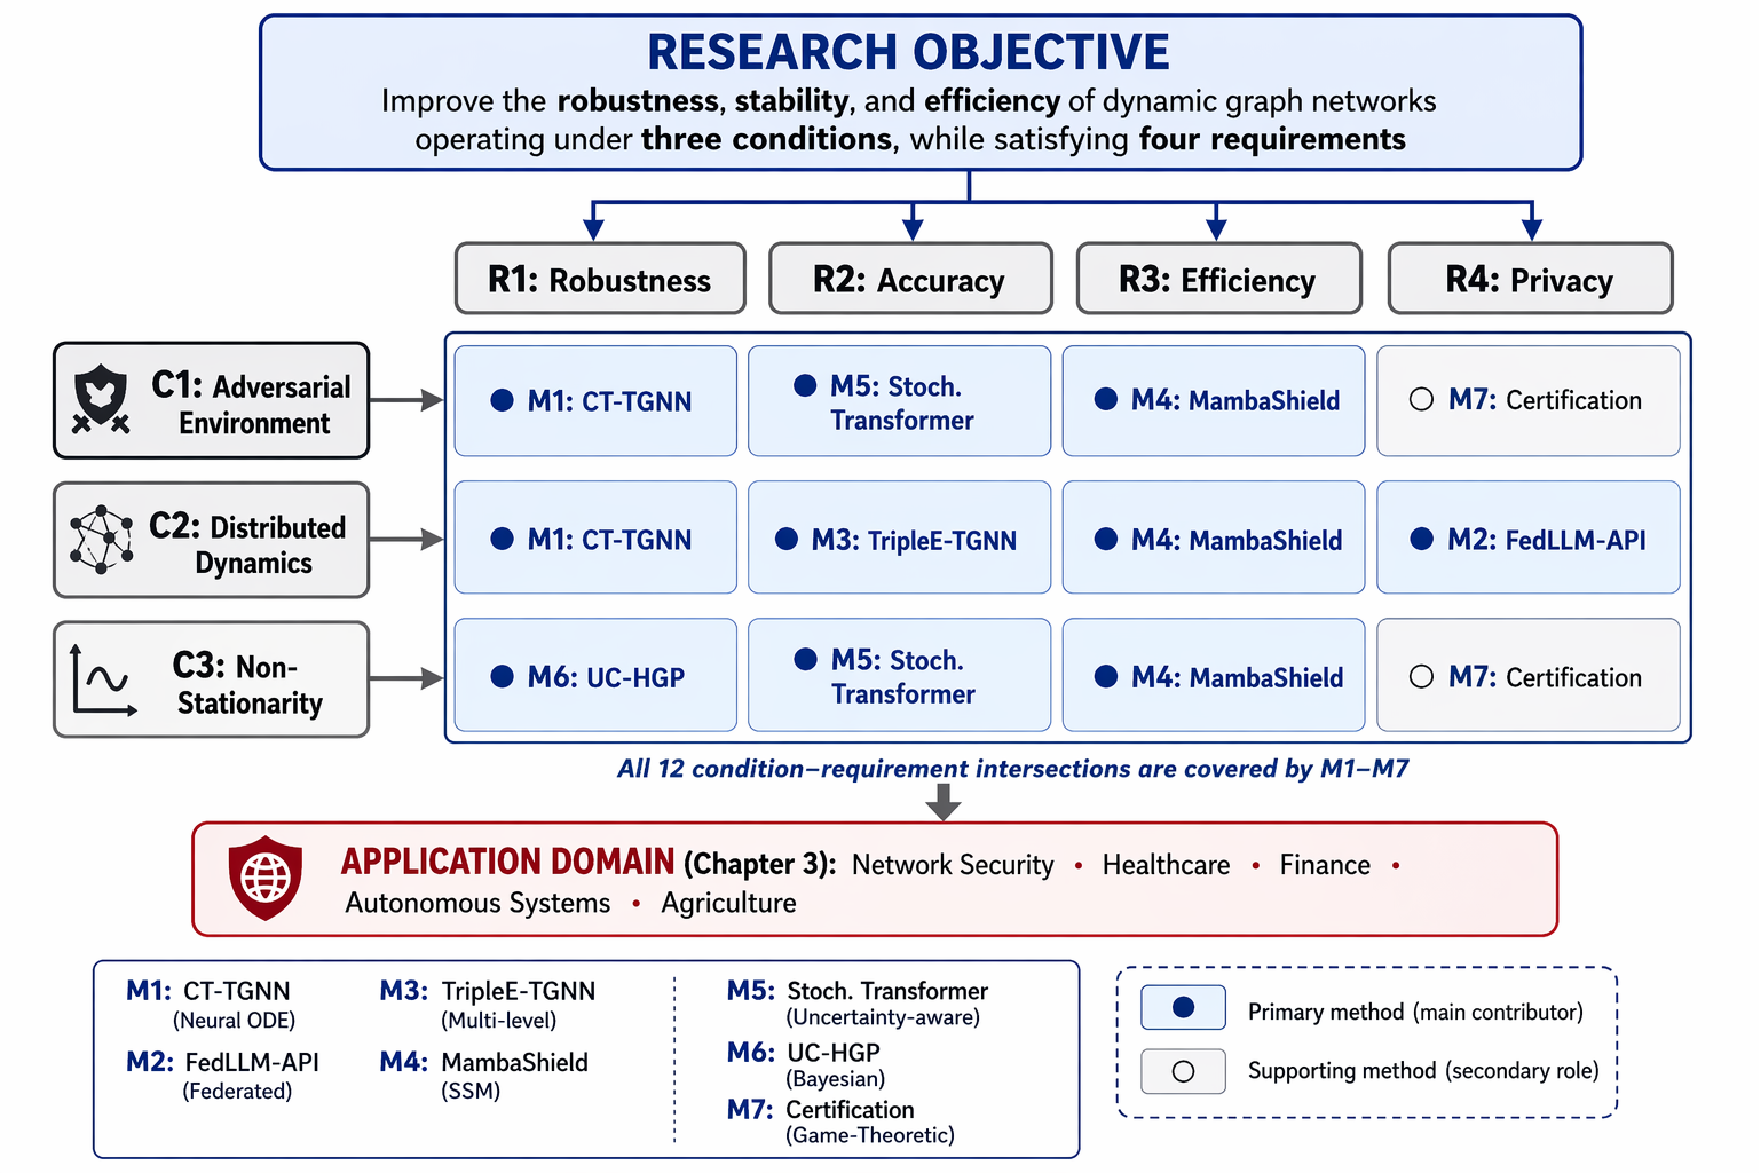
\includegraphics[width=0.95\linewidth]{figures/Main_arch_v1.pdf}
\end{center}
\smallskip
\textbf{Семь моделей M1--M7 покрывают все 12~пересечений}
матрицы <<3~условия $\times$~4~требования>> Hybrid IDPS.
Каждая сформулирована на уровне математических операций
над графовыми структурами~--- \hl{предметно-независимо}.
\end{frame}

% ============================================================
% Slide 16: Пространство задач: Венн + матрица
% ============================================================
\begin{frame}{Пространство задач Hybrid IDPS: условия и требования}
\begin{columns}[T,onlytextwidth]
\column{0.50\textwidth}
\textbf{Венн-диаграмма покрытия:}\\[2pt]
\begin{tikzpicture}[scale=0.75,transform shape]
\fill[navy!15,opacity=0.6] (0,0) circle (1.4);
\fill[good!15,opacity=0.6] (1.6,0) circle (1.4);
\fill[accent!15,opacity=0.6] (0.8,-1.3) circle (1.4);
\node at (-0.5,0.8) {\scriptsize Adversarial};
\node at (2.1,0.8) {\scriptsize Non-Stat.};
\node at (0.8,-2.4) {\scriptsize Distributed};
\node[draw=navy,fill=white,rounded corners,inner sep=1pt,font=\tiny]
  at (0.8,0.0) {CT-/SDE-TGNN, MambaShield};
\node[draw=navy,fill=white,rounded corners,inner sep=1pt,font=\tiny]
  at (-0.3,-0.5) {Stoch.\ Transf.};
\node[draw=navy,fill=white,rounded corners,inner sep=1pt,font=\tiny]
  at (2.2,-0.5) {TripleE-TGNN};
\node[draw=navy,fill=white,rounded corners,inner sep=1pt,font=\tiny]
  at (0.8,-1.7) {FedLLM-API};
\end{tikzpicture}

\column{0.50\textwidth}
\textbf{Матрица условие--требование:}\\[2pt]
\scriptsize
\begin{tabular}{@{}p{1.2cm}|p{1.3cm}p{1.3cm}p{1.3cm}@{}}
\toprule
 & \bn{Adv} & \bn{Non-St} & \bn{Distr} \\
\midrule
Acc & CT-TGNN & TripleE & FedLLM \\
Rob & SDE-TGNN & UC-HGP & FedLLM \\
Eff & MambaSh & MambaSh & OT-accel \\
Priv & FedGTD & PQC fwd & ДП $\varepsilon{=}0{,}85$\\
\bottomrule
\end{tabular}
\end{columns}
\medskip
\begin{alertblock}{}
\small Все модели в этой матрице~--- CT-TGNN, SDE-TGNN,
FedLLM-API, MambaShield и др.~--- разработаны автором и
описаны в 18~рецензируемых публикациях.
\end{alertblock}
\end{frame}

% ============================================================
% Slide 17: Объект и предмет исследования
% ============================================================
\begin{frame}{Объект и предмет исследования}
\vspace{0.4cm}
\begin{block}{Объект исследования}
\textbf{Гибридные системы обнаружения и предотвращения
вторжений (Hybrid IDPS)}, функционирующие в состязательном,
нестационарном и распределённом окружении и адаптируемые к
различным предметным областям (защита сетевого трафика,
бортовых систем БПЛА, банковской инфраструктуры,
медицинских данных, промышленного IoT и др.).
\end{block}
\medskip
\begin{block}{Предмет исследования}
\textbf{Модели, алгоритмы и специальное математическое
обеспечение} повышения \hl{робастности}, \hl{эффективности},
\hl{дифференциальной приватности} и \hl{точности}
обучаемых компонентов Hybrid IDPS, функционирующих в
состязательном, нестационарном и распределённом окружении.
\end{block}
\end{frame}

% ============================================================
% Slide 18: Цель работы
% ============================================================
\begin{frame}{Цель работы}
\vspace{1.2cm}
\begin{block}{}
\centering\large
Повысить \hl{робастность} и \hl{эффективность} гибридных
систем обнаружения и предотвращения вторжений (Hybrid IDPS),
функционирующих в \bn{состязательных, нестационарных и
распределённых} условиях, путём разработки единого
математического описания Hybrid IDPS и семейства согласованных
моделей и алгоритмов с формальными гарантиями.
\end{block}
\vspace{0.6cm}
\begin{center}
\textit{Каковы задачи для достижения этой цели?}
\end{center}
\end{frame}

% ============================================================
% Slide 19: Задачи
% ============================================================
\begin{frame}{Задачи для достижения цели}
\scriptsize
\begin{enumerate}
\item Систематизировать существующие подходы к Hybrid IDPS
в 7~прикладных секторах, выявить пробелы и сформулировать
требования к разрабатываемым моделям и алгоритмам.

\item Сформировать единое математическое описание Hybrid IDPS
в виде кортежа $\mathcal{H}=(\mathcal{V}_t,\mathcal{E}_t,X_t,A_t,
f_\theta,g_\psi,\pi)$ и шести инвариантных свойств P1--P6,
образующих $3\times4$ матрицу <<условия$\times$требования>>.

\item Разработать 7~моделей и алгоритмов M1--M7, покрывающих
все 12~ячеек матрицы: CT-TGNN/SDE-TGNN~(M1), FedLLM-API~(M2),
TripleE-TGNN~(M3), MambaShield~(M4),
Stoch.Transf./UC-HGP~(M5--M6), FedGTD-сертификация~(M7).

\item Инстанцировать Hybrid IDPS в NIDPS-секторе: формальный
конвейер <<данные$\to$граф>>, унифицированная таксономия из
34~классов атак, 83~инженерных признака.

\item Провести экспериментальную валидацию на 6~эталонных
наборах данных (84,2~млн образцов, 84~категории, 23~метрики)
с превосходством над базовыми методами на 2,9--5,6~п.\,п.

\item Реализовать программную платформу промышленного уровня
\bn{RobustIDPS.ai} (\hl{17~моделей в 10~функциональных
группах}, 51~страница) с четырёхуровневой защитой LLM
(94,5\% по 517 сценариям) и подтвердить актами от четырёх
организаций.

\item Применить единую систему и продемонстрировать её
качество в смежном секторе защиты бортовых систем БПЛА
(<<борт~-- дронопорт~-- облако>>) и кросс-доменно (речь,
медицина).
\end{enumerate}
\end{frame}

% ============================================================
% Slide 20: Научная новизна
% ============================================================
\begin{frame}{Научная новизна}
\scriptsize
\begin{enumerate}
\item \bn{Впервые} построено единое математическое описание
\hl{Hybrid IDPS} в виде кортежа
$\mathcal{H}=(\mathcal{V}_t,\mathcal{E}_t,X_t,A_t,f_\theta,
g_\psi,\pi)$ и системы шести инвариантных свойств P1--P6.

\item \bn{Впервые} в составе Hybrid IDPS установлен принцип
сертифицированной устойчивости непрерывно-временной графовой
динамики (CT-TGNN, SDE-TGNN)~--- границы Гр\"енуолла и
аналитическое распространение моментов через уравнение
Фоккера--Планка.

\item \bn{Оригинальная} теория совместного обеспечения
византийской устойчивости, формальной приватности и
распределительного выравнивания при обучении обучаемых
компонентов Hybrid IDPS на разрозненных графовых фрагментах
(FedLLM-API).

\item \bn{Новая} концепция многоуровневого графового
представления (TripleE-TGNN) с защитой от утраты ранее
усвоенных закономерностей при поступлении новых данных.

\item \bn{Новый} подход к эффективному выводу обучаемых
компонентов Hybrid IDPS на основе селективных пространств
состояний (MambaShield, $\mathcal{O}(L\log L)$).

\item \bn{Впервые} в составе Hybrid IDPS предложена интегрированная
теория калиброванной неопределённости (Stoch.\ Transformer,
UC-HGP) с эпистемически-алеаторной декомпозицией.

\item \bn{Оригинальная} концепция единой сертификации Hybrid
IDPS (FedGTD), где взаимодействие защитника и противника
моделируется как стратегическая игра с доказуемо оптимальной
стратегией выбора.

\item \bn{Новая} теория предметно-ориентированного фундаментального
моделирования на графовых структурах (CyberSecLLM) с
распознаванием ранее невиданных категорий угроз.
\end{enumerate}
\end{frame}

% ============================================================
% Slide 21: Соответствие П.4
% ============================================================
\begin{frame}{Соответствие паспорту специальности~--- П.4}
{\footnotesize Специальность 2.3.1: <<Системный анализ,
управление и обработка информации, статистика>>}
\smallskip

\textbf{П.4:} Разработка \emph{методов и алгоритмов} решения
задач системного анализа, оптимизации, управления, принятия
решений, обработки информации и искусственного интеллекта.
\medskip

\scriptsize
\begin{tabular}{p{3.6cm}p{8.0cm}}
\toprule
\textbf{Требование П.4} & \textbf{Вклад диссертации} \\
\midrule
Методы системного анализа & Единая матрица $3\times4$
<<условия$\times$требования>>, декомпозирующая проблему
устойчивости Hybrid IDPS на 7 подзадач \\
\midrule
Алгоритмы оптимизации & Адъюнктное обучение CT-TGNN,
БПФ-свёртки MambaShield, византийски-устойчивая FedLLM-API \\
\midrule
Принятие решений & Теоретико-игровые равновесия Штакельберга
(M7) для выбора стратегии защитника с гарантиями отсутствия
сожаления \\
\midrule
Обработка информации & Конвейер извлечения 83~признаков,
обработка 84,2~млн размеченных образцов по 6 наборам данных \\
\midrule
Искусственный интеллект & 7 новых архитектур обучаемых
компонентов Hybrid IDPS (M1--M7) с 6 доказанными теоремами о
сходимости и устойчивости \\
\bottomrule
\end{tabular}
\end{frame}

% ============================================================
% Slide 22: Соответствие П.5
% ============================================================
\begin{frame}{Соответствие паспорту специальности~--- П.5}
\textbf{П.5:} Разработка \emph{специального математического
и алгоритмического обеспечения} систем анализа, оптимизации,
управления, принятия решений, обработки информации и
искусственного интеллекта.
\medskip

\scriptsize
\begin{tabular}{p{3.6cm}p{8.0cm}}
\toprule
\textbf{Требование П.5} & \textbf{Вклад диссертации} \\
\midrule
Математическое обеспечение & Сертификаты Липшица на основе
неравенства Гр\"енуолла, распространение моментов
Фоккера--Планка, PAC-байесовские оценки,
Вассерштейновское ОТ-выравнивание \\
\midrule
Алгоритмическое обеспечение & 8 алгоритмов: обучение CT-TGNN,
сэмплирование SDE-TGNN, агрегация FedLLM-API, дистилляция
MambaShield, вывод UC-HGP, сертификация MWU, токенизация
CyberSecLLM, отклик MA-CPO \\
\midrule
Системы управления & Многоагентная ограниченная оптимизация
политики (MA-CPO) для автономного реагирования Hybrid IDPS
на угрозы без нарушения ограничений \\
\midrule
Программная реализация & Платформа \hl{RobustIDPS.ai}:
\hl{51~страница}, \hl{17~моделей}, \hl{10~функциональных
групп} (DOI:~10.5281/zenodo.19129512), интеграция со
Snort/Suricata\\
\bottomrule
\end{tabular}
\end{frame}

% ============================================================
% Slide 23: Теоретическая значимость
% ============================================================
\begin{frame}{Теоретическая значимость}
\textbf{Впервые объединены \bn{пять областей математики} для
робастного обучения в составе Hybrid IDPS на графах:}
\smallskip
\begin{columns}[T,onlytextwidth]
\column{0.50\textwidth}
\textbf{Пять теорий:}
\begin{enumerate}\setlength\itemsep{0pt}
\item \bn{Нейронные ОДУ/СДУ}~--- доказуемо ограниченная
чувствительность выхода
\item \bn{Оптимальный транспорт}~--- выравнивание данных
между организациями с гарантиями приватности
\item \bn{Пространства состояний}~--- снижение времени
обработки до почти линейного
\item \bn{Байесовский вывод}~--- Hybrid IDPS знает, когда
ему нельзя доверять
\item \bn{Теория игр}~--- оптимальная стратегия защиты от
адаптивного противника
\end{enumerate}

\column{0.50\textwidth}
\textbf{Шесть формальных гарантий:}
\begin{enumerate}\setlength\itemsep{0pt}
\item Сходимость обучения к оптимуму
\item Робастность: ограниченное изменение выхода
\item Приватность: невосстановимость личных данных
\item Обобщение: качество на невиданных данных
\item Регрет: убывание ошибки при онлайн-адаптации
\item Единая сходимость всех 7~моделей
\end{enumerate}
\smallskip
\begin{block}{}
\scriptsize Все гарантии \hl{предметно-независимы} и
подтверждены на 84,2~млн образцов.
\end{block}
\end{columns}
\end{frame}

% ============================================================
% Slide 24: Практическая значимость
% ============================================================
\begin{frame}{Практическая значимость}
\textbf{Кто может использовать, как и в какой области:}
\smallskip
\begin{columns}[T,onlytextwidth]
\column{0.48\textwidth}
\textbf{Здравоохранение:} CT-TGNN и SDE-TGNN интегрированы
в Hybrid IDPS клинических платформ поддержки решений для
сертифицированных предсказаний на молекулярных графах.\smallskip

\textbf{Финансы:} FedLLM-API позволяет банкам и регуляторам
совместно обучать Hybrid IDPS обнаружения мошенничества на
графах транзакций без обмена данными клиентов.\smallskip

\textbf{Промышленный IoT:} MambaShield развёрнут на
периферийных шлюзах и SCADA-контроллерах для обнаружения
аномалий в реальном времени.

\column{0.48\textwidth}
\textbf{Автономные системы:} UC-HGP обеспечивает инженеров
безопасности БПЛА эпистемическими оценками уверенности
Hybrid IDPS для решений по слиянию датчиков.\smallskip

\textbf{Кибербезопасность:} \bn{RobustIDPS.ai} (DOI:
10.5281/zenodo.19129512) непосредственно используется
SOC-аналитиками, инженерами кибербезопасности, исследователями
MLSecOps~--- разработан как \hl{плагин для Snort и Suricata}.\smallskip

\begin{alertblock}{4 акта внедрения}
\small Росатом~|~Positive~Technologies~|~GCP~|~Suricata
\end{alertblock}
\end{columns}
\end{frame}

% ============================================================
% Slide 25: Личный вклад (1/2)
% ============================================================
\begin{frame}{Личный вклад (1/2)}
\small
Все результаты получены автором \hl{лично} под научным
руководством проф.\ А.\,Г.~Трофимова.

\begin{enumerate}
\item \bn{Лично} построил единое математическое описание
Hybrid IDPS в виде кортежа $\mathcal{H}$ и системы шести
инвариантных свойств P1--P6, обосновав построение семейства
M1--M7 как покрытия матрицы $3\times4$.

\item \bn{Лично} разработал архитектуры CT-TGNN и SDE-TGNN~---
первые модели в составе Hybrid IDPS, в которых эволюция узлов
графа управляется дифференциальными уравнениями непрерывного
времени с доказанными границами устойчивости.

\item \bn{Лично} создал алгоритм FedLLM-API~--- федеративный
оптимизатор, обеспечивающий совместное обучение между
организациями Hybrid IDPS без передачи данных, с защитой от
злонамеренных участников и формальными гарантиями приватности.

\item \bn{Лично} спроектировал архитектуру TripleE-TGNN~---
трёхуровневую систему представления графов Hybrid IDPS,
предотвращающую забывание ранее изученных паттернов при
обучении на новых данных.
\end{enumerate}
\end{frame}

% ============================================================
% Slide 26: Личный вклад (2/2)
% ============================================================
\begin{frame}{Личный вклад (2/2)}
\small
\begin{enumerate}\setcounter{enumi}{4}
\item \bn{Лично} разработал модель MambaShield~--- эффективную
архитектуру для обучаемых компонентов Hybrid IDPS, ускоряющую
обработку данных с квадратичной до почти линейной сложности,
устойчивую к отравлению обучающих данных.

\item \bn{Лично} интегрировал Stochastic Transformer и
UC-HGP~--- систему, позволяющую обучаемому компоненту Hybrid
IDPS сообщать, когда он не уверен в своём решении, и
автоматически адаптироваться к изменяющимся условиям.

\item \bn{Лично} построил единую систему сертификации
FedGTD~--- связал все 7~моделей через теоретико-игровой
подход и валидировал на 84,2~миллионах образцов.

\item \bn{Лично} реализовал платформу \hl{RobustIDPS.ai}~---
\hl{51~страница}, \hl{17~моделей в 10~функциональных группах},
внедрение в 4~организациях.
\end{enumerate}
\smallskip
\begin{block}{}
\small\textbf{Вклад автора составляет 100\%} в постановке
задач, разработке моделей, проведении экспериментов, создании
программного обеспечения и подготовке публикаций.
\end{block}
\end{frame}

% ============================================================
% Slide 27: Публикации: журнальные статьи
% ============================================================
\begin{frame}{Публикации: журнальные статьи}
\scriptsize
\begin{tabular}{cclll}
\toprule
\# & Год & Название (кратко) & Журнал & Индекс \\
\midrule
1 & 2026 & MambaShield: селективные SSM для Hybrid IDPS & Expert Syst.\ Appl. & Q1/Scopus/WoS \\
2 & 2026 & Калиброванные иерархические ГП для IDPS & Neurocomputing & Q1/Scopus/WoS \\
3 & 2026 & Временные адаптивные ОДУ для NIDPS & Complex Intell.\ Syst. & Q1/Scopus/WoS \\
4 & 2024 & Улучшенная состязательная модель IDS & Opt.\ Mem.\ Neural Net. & Q3/Scopus/WoS \\
\midrule
\multicolumn{5}{l}{\textit{Принятые к публикации:}} \\
5 & 2025 & PAC-байесовские трансформеры для NIDS и NLP & Knowl.\ Inf.\ Syst. & Q1/Scopus/WoS \\
6 & 2026 & Виз.\ устойчивые стохаст.\ игры для фед.\ IDPS & Complex Intell.\ Syst. & Q1/Scopus/WoS \\
\bottomrule
\end{tabular}
\medskip
\begin{block}{}
\small \hl{6 журнальных статей} (4 опубликованных + 2
принятых) в журналах Scopus/Web of Science. Издательства:
Elsevier~(2), Springer~(4).
\end{block}
\end{frame}

% ============================================================
% Slide 28: Публикации: труды конференций
% ============================================================
\begin{frame}{Публикации: труды конференций}
\scriptsize
\begin{tabular}{cclll}
\toprule
\# & Год & Название (кратко) & Конференция & Индекс \\
\midrule
7 & 2025 & Стохастический мультимодальный трансформер & NEUROINFORMATICS 2025 & Springer \\
8 & 2025 & DQN и актор-критик для атак отравления в NIDS & ElCon 2025, С-Петербург & IEEE Xplore \\
9 & 2024 & Модели МО для идентификации устройств & ElCon 2024, С-Петербург & IEEE Xplore \\
\midrule
\multicolumn{5}{l}{\textit{Предстоящие доклады (2026):}} \\
10 & Июнь 2026 & EDM-2026 (27-я IEEE) & Республика Алтай & IEEE \\
11 & Сент.\ 2026 & IEEE ESTC 2026 & Хельсинки, Финляндия & IEEE \\
12 & Окт.\ 2026 & IEEE RTSI 2026 & Эспоо, Финляндия & IEEE \\
13 & Дек.\ 2026 & NeurIPS 2026 (40-я) & Сидней, Австралия & PMLR \\
\bottomrule
\end{tabular}
\medskip
\begin{block}{}
\small\textbf{Итого: 18 публикаций и докладов}~--- 6~журнальных
статей + 3~опубликованных труда конференций + 4~предстоящих
доклада + 5~статей на рецензировании в IEEE~Trans.
\end{block}
\end{frame}

% ============================================================
% Slide 29: Chapter 1 divider
% ============================================================
\begin{frame}{1: Обзор литературы и анализ пробелов}
\vspace{1.5cm}
\begin{center}
{\Large\bn{Анализ Hybrid IDPS в семи прикладных секторах,\\
структурных проблем и теоретических основ}}\\[1cm]

Систематический обзор в соответствии с охватом исследования:\\
\textit{Hybrid IDPS $\to$ Динамика НВ $\to$ Распределённость
$\to$ Эффективность $\to$ Нестационарность}\\[0.5cm]

Все 12 пересечений матрицы $3\times4$ покрыты\\[0.4cm]

\textcolor{accent}{\textbf{7 исследовательских пробелов
выявлены из 128 цитируемых работ}}
\end{center}
\end{frame}

% ============================================================
% Slide 30: Уязвимость обучаемых компонентов Hybrid IDPS
% ============================================================
\begin{frame}{Уязвимость обучаемых компонентов Hybrid IDPS: двойная поверхность атаки}
\begin{columns}[T,onlytextwidth]
\column{0.50\textwidth}
Обучаемые компоненты Hybrid IDPS принимают \hl{два входа}:
\begin{itemize}
\item Данные $X\in\mathbb{R}^{n\times d}$ (матрица признаков:
$n$ узлов, $d$ атрибутов)
\item Структура $A\in\{0,1\}^{n\times n}$ (матрица смежности:
кто с кем связан)
\end{itemize}
Возмущение любого из них нарушает выход контура Hybrid IDPS.
\smallskip

\textbf{Задокументированные отказы Hybrid IDPS:}
\begin{itemize}\setlength\itemsep{0pt}
\item Здравоохранение: 25\% падение AUC
\item Финансы: 25,7\%~$\to$~68,6\% ошибок
\item Промышленность: 94,2\%~$\to$~30\% коллапс
\item Кибербезопасность: $-$59\% обнаружения
\end{itemize}

\column{0.50\textwidth}
\textbf{Существующие границы устойчивости} (Gama и др.):
растут с глубиной; не распространяются на темпоральные или
состязательные условия Hybrid IDPS.
\smallskip

\begin{block}{Ключевая идея: граница Гр\"енуолла}
\[
\|h_1(T)-h_2(T)\| \le e^{L_g T}\|x_1-x_2\|
\]
\end{block}
\smallskip
\scriptsize
\begin{tabular}{ll}
$h_i(T)$ & выходное вложение в момент $T$ \\
$x_i$ & вход (признаки + структура) \\
$L_g$ & константа Липшица (гладкость) \\
$e^{L_g T}$ & макс.\ коэффициент усиления \\
\end{tabular}
\smallskip
\begin{alertblock}{}
\scriptsize Ни одна существующая работа не использует эту
оценку в составе Hybrid IDPS для эволюционирующих графов.
\end{alertblock}
\end{columns}
\end{frame}

% ============================================================
% Slide 31: 7 нерешённых пробелов
% ============================================================
\begin{frame}{Пробелы в литературе: 7 нерешённых проблем Hybrid IDPS}
\scriptsize
\begin{columns}[T,onlytextwidth]
\column{0.48\textwidth}
\textbf{Состязательность (Пробел 1):}
Нет сертифицированных границ робастности на основе динамики
ОДУ непрерывного времени для эволюционирующих топологий
графов Hybrid IDPS.\smallskip

\textbf{Распределённость (Пробел 2):}
Нет алгоритма, одновременно гарантирующего византийскую
устойчивость + дифф.\ приватность + ОТ-выравнивание для
графовых данных Hybrid IDPS.\smallskip

\textbf{Эффективность (Пробелы 3--4):}
Нет многоуровневых темпоральных вложений графов с защитой от
забывания; модели пространства состояний не адаптированы для
графов с гарантиями робастности.

\column{0.48\textwidth}
\textbf{Нестационарность (Пробелы 5--6):}
Нет прямо совместимого обнаружения при смене протокольного
режима (постквантовый); нет интегрированного байесовского
внимания + гауссовских процессов для графов Hybrid IDPS.\smallskip

\textbf{Сертификация (Пробел 7):}
Нет единой системы, сочетающей теорию игр, интервальные
границы, анализ Липшица и рандомизированное сглаживание для
графов в составе Hybrid IDPS.\smallskip

\begin{alertblock}{}
\scriptsize Все 7 пробелов $\to$ 7 моделей (M1--M7) покрывают
все 12 ячеек матрицы условие--требование Hybrid IDPS.
\end{alertblock}
\end{columns}
\end{frame}

% ============================================================
% Slide 32: Сводка 7 пробелов
% ============================================================
\begin{frame}{Сводка 7 исследовательских пробелов}
\small
\begin{tabular}{clll}
\toprule
\# & Описание пробела & Усл. & Предлож.\ метод \\
\midrule
1 & Нет сертиф.\ НВ робастности графов Hybrid IDPS & У1, У2 & M1: CT-TGNN/SDE-TGNN \\
2 & Приватность-качество в федерат.\ Hybrid IDPS & У3 & M2: FedLLM-API \\
3 & Нет многоуровн.\ моделей без забывания & У2 & M3: TripleE-TGNN \\
4 & Квадратич.\ стоимость, нет робаст.\ SSM & У1, У2 & M4: MambaShield \\
5 & Прямая несовместимость новых угроз & У2 & CyberSecLLM \\
6 & Неинтегрированная неопределённость & У1, У2 & M5/M6: Stoch.\ Tr.\ + UC-HGP \\
7 & Упрощённые модели угроз & Все & M7: FedGTD-сертификация \\
\bottomrule
\end{tabular}
\medskip

\scriptsize У1: Состязательная среда~~|~~У2: Нестационарность~~|~~У3: Распределённая динамика
\smallskip

\begin{alertblock}{}
\small Все 12 ячеек матрицы $3\times4$ условие--требование
Hybrid IDPS \hl{покрыты} семейством M1--M7.
\end{alertblock}
\end{frame}

% ============================================================
% Slide 33: Key inference Ch1 -> Ch2
% ============================================================
\begin{frame}{Ключевой вывод Главы 1~$\to$~Главе 2}
\begin{block}{1: Обзор литературы}
\small Выявлено \hl{7 конкретных нерешённых пробелов} Hybrid
IDPS в областях динамики непрерывного времени, распределённого
обучения, эффективности, нестационарности и единой
сертификации. Каждый пробел подтверждён данными из
\hl{128 цитируемых работ}.
\end{block}
\smallskip
\centering
\textcolor{accent}{\textbf{$\Rightarrow$ Глава 2 разрабатывает
единое математическое описание Hybrid IDPS и семейство
M1--M7 для заполнения этих пробелов.}}\smallskip

\begin{block}{2: Модели и алгоритмы}
\small
Единая постановка задачи $\to$ 7 подзадач $\to$ 7 моделей\\
\textbf{62 уравнения~|~6 теорем~|~8 алгоритмов}\\
Последовательный вывод:\\
база $\to$ состязательность $\to$ ОДУ $\to$ федерат.\
$\to$ многоуровн.\ $\to$ SSM $\to$ регрет
\end{block}
\end{frame}

% ============================================================
% Slide 34: Единая постановка задачи
% ============================================================
\begin{frame}{Единая постановка задачи Hybrid IDPS (последовательный вывод)}
\scriptsize
Каждый этап добавляет ограничение; каждый порождает подзадачу
для конкретного компонента Hybrid IDPS, решаемую конкретным
методом:
\smallskip
\begin{enumerate}
\item \textbf{Базовая классификация:} $\min_\theta\mathbb{E}[\mathcal{L}(f_\theta(\mathcal{G}),y)]$ \\
{\scriptsize Минимизировать ожидаемые потери $\mathcal{L}$ модели $f_\theta$ на графе $\mathcal{G}$ с меткой $y$}

\item \textbf{+ Состязательность (P1):} $\max_{\|\delta\|\le\epsilon}\mathcal{L}(f_\theta(\mathcal{G}+\delta),y)$\\
{\scriptsize Наихудшее возмущение $\delta$ в пределах бюджета $\epsilon$}

\item \textbf{+ Ограничение ОДУ (M1):} $dh/dt=f_\theta(h,A,t)$, Липшиц $\le L_g$ \\
{\scriptsize Состояния узлов $h$ эволюционируют через ОДУ с ограниченной гладкостью $L_g$}

\item \textbf{+ Приватность (M2):} $\Pr[\mathcal{M}(D)\in S]\le e^\varepsilon\Pr[\mathcal{M}(D')\in S]+\delta$\\
{\scriptsize Механизм обучения скрывает любую отдельную запись данных (бюджет $\varepsilon$)}

\item \textbf{+ Многоуровневость (M3):} $h_k=\bar{A}(u_k)h_{k-1}+\bar{B}(u_k)x_k$ за $\mathcal{O}(L\log L)$ \\
{\scriptsize Трёхуровневые потери со штрафом Фишера $F_i$, предотвращающим забывание}

\item \textbf{+ Эффективность (M4):} $h_k=\bar{A}(u_k)h_{k-1}+\bar{B}(u_k)x_k$ за $\mathcal{O}(L\log L)$\\
{\scriptsize Рекуррентность пространства состояний через БПФ, заменяющая внимание $\mathcal{O}(L^2)$}

\item \textbf{+ Регрет (M5/M6/M7):} $R(T)\le\mathcal{O}(\sqrt{T\log|S|})$\\
{\scriptsize Онлайн-адаптация с убывающим средним регретом $R(T)/T\to0$}
\end{enumerate}
\end{frame}

% ============================================================
% Slide 35: M1: CT-TGNN
% ============================================================
\begin{frame}{M1: CT-TGNN~--- сертифицированная динамика непрерывного времени в Hybrid IDPS}
\begin{columns}[T,onlytextwidth]
\column{0.50\textwidth}
\scriptsize
\textbf{Нейронное ОДУ на эволюционирующем графе Hybrid IDPS:}
\[
\frac{dh_v(t)}{dt}=f_\theta(h_v(t),\mathcal{N}_v(t),A(t),t)
\]
\begin{itemize}
\item $h_v(t)$: вложение узла $v$
\item $\mathcal{N}_v(t)$: соседи в момент $t$
\item $A(t)$: структура графа в момент $t$
\item $f_\theta$: обученная функция динамики
\end{itemize}
\smallskip
\textbf{Многомасштабность:} 3 ветви
$\tau_1{=}1$\,c (пакеты), $\tau_2{=}60$\,c (сессии),
$\tau_3{=}3600$\,c (кампании)\smallskip

\textbf{Сопряжённое обучение:} $\mathcal{O}(1)$ памяти\\
\textbf{TABN:} темпоральная адаптивная пакетная нормализация\smallskip

\textbf{Теорема (Сертификат Липшица):}
$\|h_1(T)-h_2(T)\| \le e^{L_g T}\|x_1-x_2\|$\\
\textbf{Теорема (Сходимость):} $\mathcal{O}(1/\sqrt{T})$

\column{0.50\textwidth}
\centering
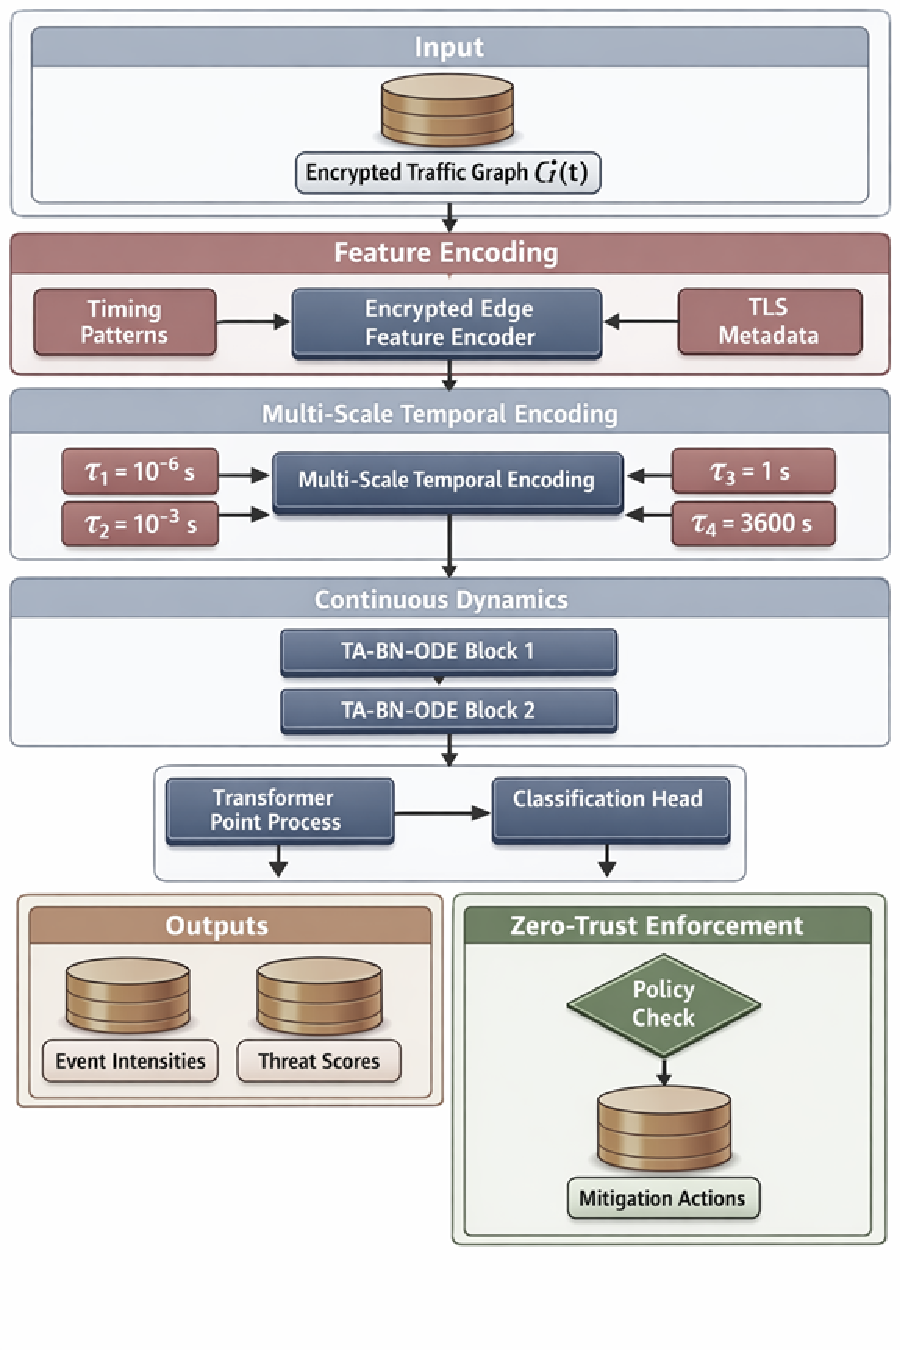
\includegraphics[width=0.95\linewidth]{figures/fig_CT-TGNN_architecture.pdf}\\[2pt]
{\scriptsize Архитектура CT-TGNN: три ветви ОДУ на разных
временных масштабах в составе Hybrid IDPS, объединённые
TABN и взвешенным вниманием}
\end{columns}
\end{frame}

% ============================================================
% Slide 36: M2 + M3
% ============================================================
\begin{frame}{M2: FedLLM-API~+~M3: TripleE-TGNN}
\begin{columns}[T,onlytextwidth]
\column{0.50\textwidth}
\scriptsize
\textbf{M2: FedLLM-API (Пробел 2)}
\begin{itemize}\setlength\itemsep{0pt}
\item Византийская агрегация усечённым средним
\item ($\varepsilon{=}0{,}85$, $\delta{=}10^{-5}$) ДП
\item Выравнивание ОТ Вассерштейна
\item Ветвь LLM zero-shot ($\lambda_{\text{LLM}}{=}0{,}3$)
\end{itemize}
\textbf{Теорема:} $\mathcal{O}(1/\sqrt{T})$ сходимость при 30\% повреждённых\smallskip

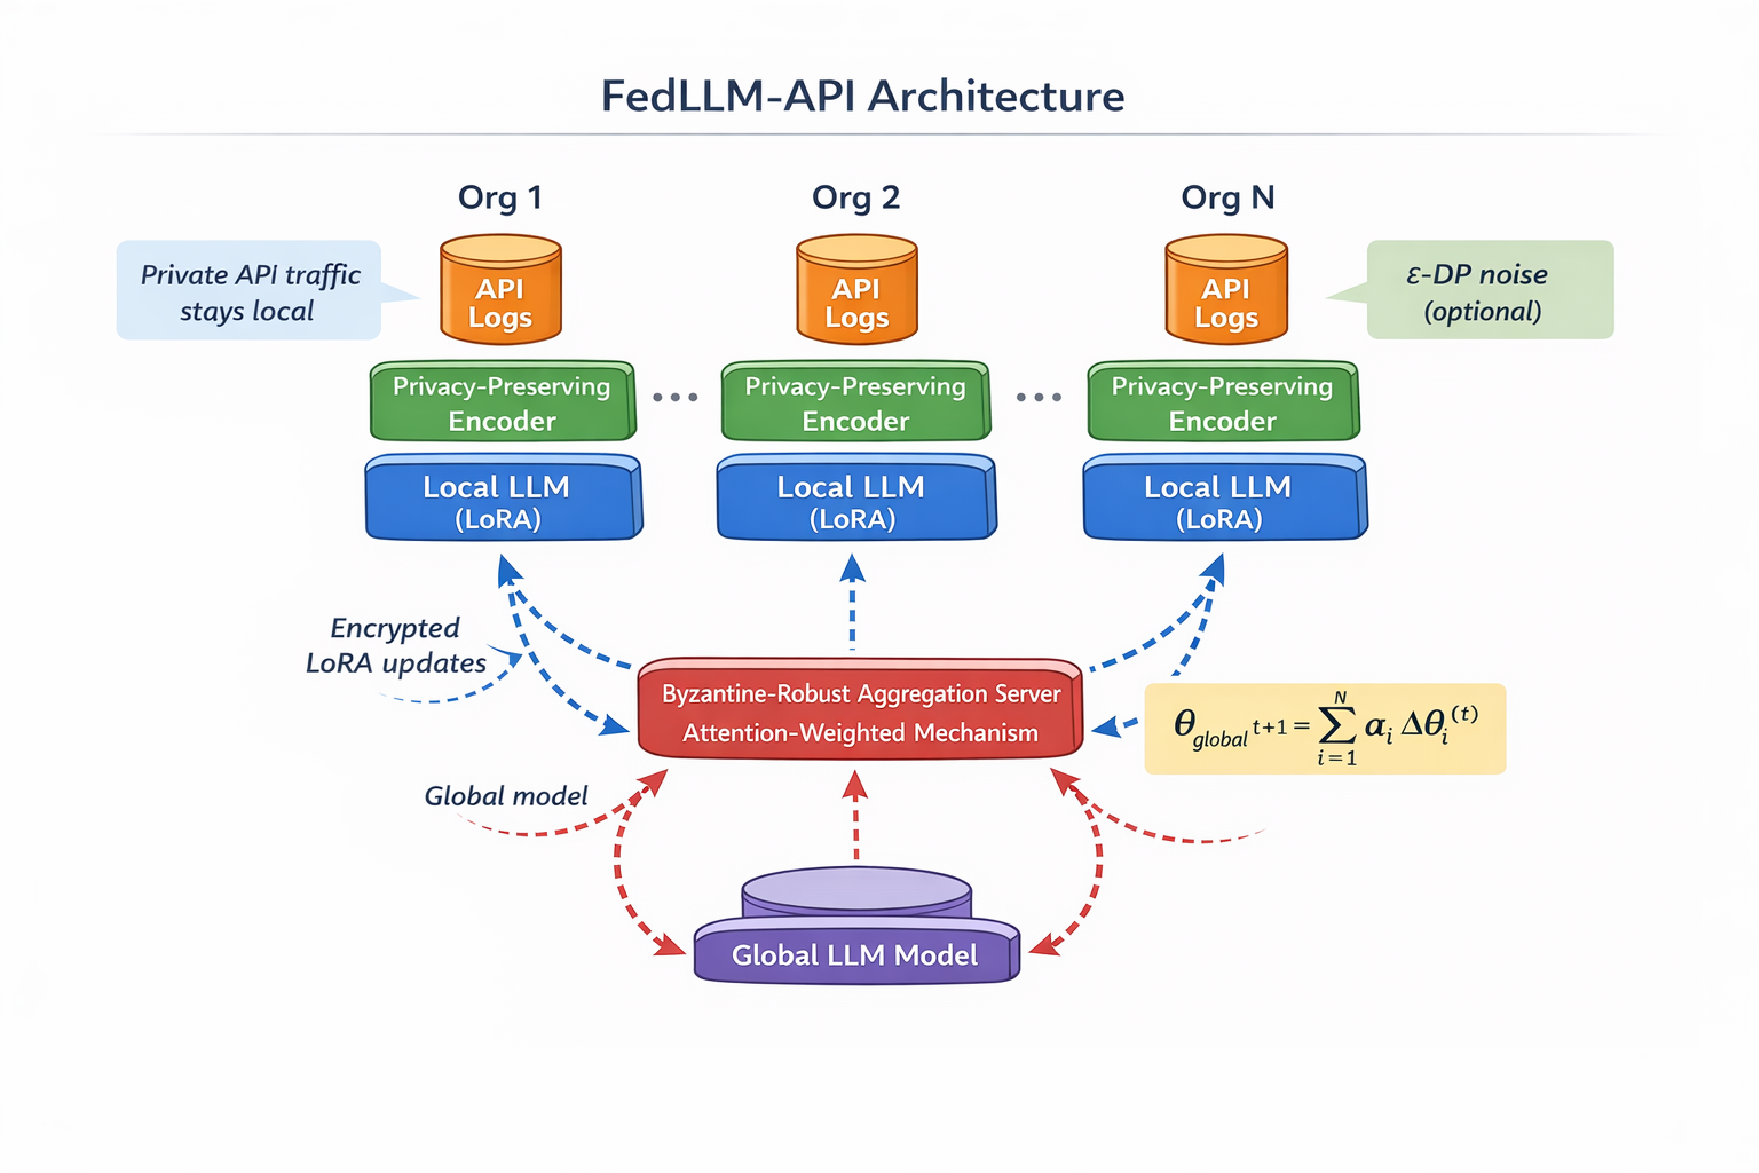
\includegraphics[width=\linewidth]{figures/fig_fedllm_api_architecture.pdf}

\column{0.50\textwidth}
\scriptsize
\textbf{M3: TripleE-TGNN (Пробел 3)}
\begin{itemize}\setlength\itemsep{0pt}
\item Вложения сервисов/трассировок/узлов
\item Двойное темпорально-пространств.\ внимание
\item EWC против забывания ($\lambda_{\text{ewc}}{=}0{,}5$)
\item Межуровневая KL-согласованность
\end{itemize}
\textbf{Многозадачность:}
$\mathcal{L}_{\text{joint}}=\sum_g\lambda_g\mathcal{L}_g+\lambda_{\text{con}}\mathcal{L}_{\text{consist}}$\smallskip

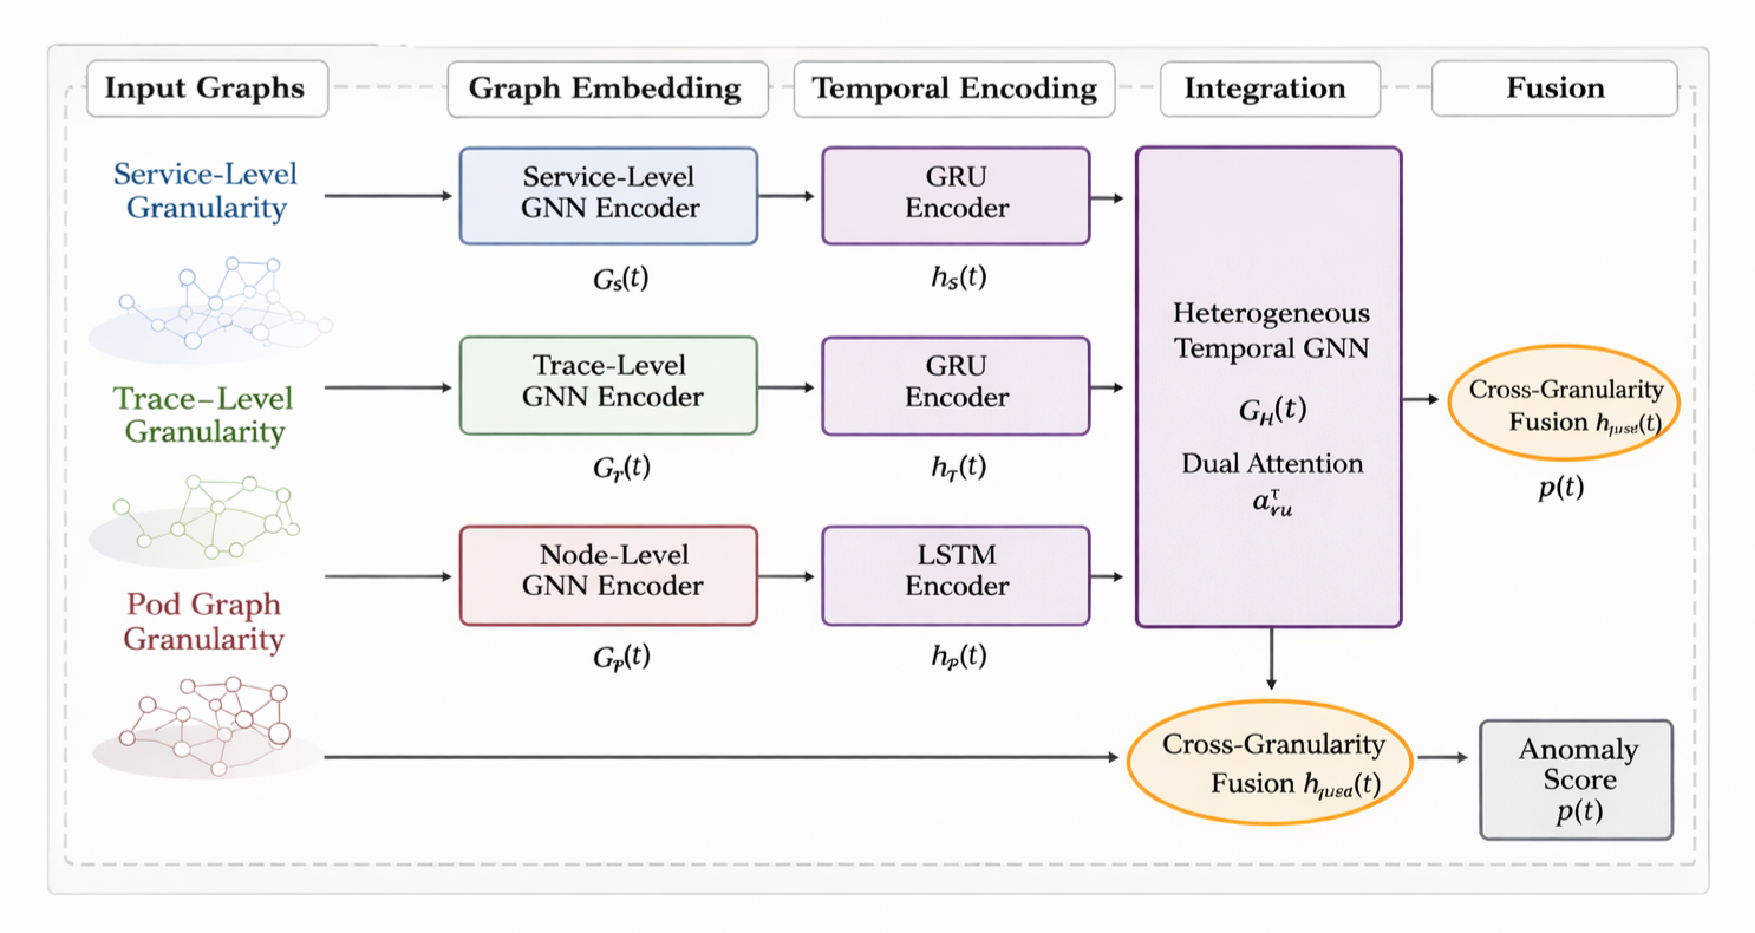
\includegraphics[width=\linewidth]{figures/fig_triplee_tgnn_architecture.pdf}
\end{columns}
\end{frame}

% ============================================================
% Slide 37: M4 + M5/M6
% ============================================================
\begin{frame}{M4: MambaShield~+~M5/M6: Неопределённость}
\begin{columns}[T,onlytextwidth]
\column{0.50\textwidth}
\scriptsize
\textbf{M4: MambaShield (Пробел 4)}
\begin{itemize}\setlength\itemsep{0pt}
\item Селективный SSM: $\mathcal{O}(L^2)\to\mathcal{O}(L\log L)$
\item Ядро свёртки БПФ
\item Прогрессивная состязательная дистилляция
\item PAC-байесовский сертификат
\end{itemize}
\smallskip
\textbf{Теорема:}\\
$\displaystyle R(\theta)\le\hat{R}_n+\sqrt{\frac{\mathrm{KL}(Q\|P)+\ln(2\sqrt{n}/\delta)}{2n}}$
\smallskip
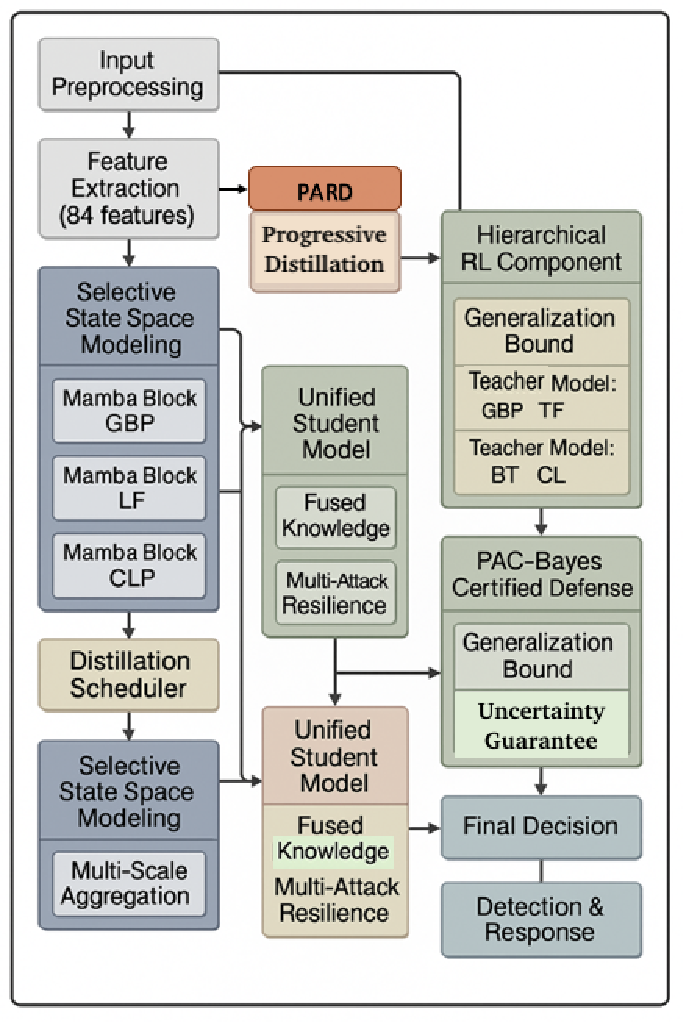
\includegraphics[width=0.85\linewidth]{figures/fig_mambashield_architecture.pdf}

\column{0.50\textwidth}
\scriptsize
\textbf{M5/M6: Сточ.\ трансф.\ + UC-HGP (Пробел 6)}
\begin{itemize}\setlength\itemsep{0pt}
\item Вариационное байесовское внимание
\item $M{=}50$ прямых проходов МК
\item Декомпозиция эпистемич.--алеаторн.\ неопр.
\item Стохастическое состязательное обучение
\end{itemize}
\smallskip
\[
\begin{aligned}
U_{\text{epi}}&=\mathrm{Var}_\theta[\mathbb{E}[y|x,\theta]]\\
U_{\text{ale}}&=\mathbb{E}_\theta[\mathrm{Var}[y|x,\theta]]
\end{aligned}
\]
\smallskip
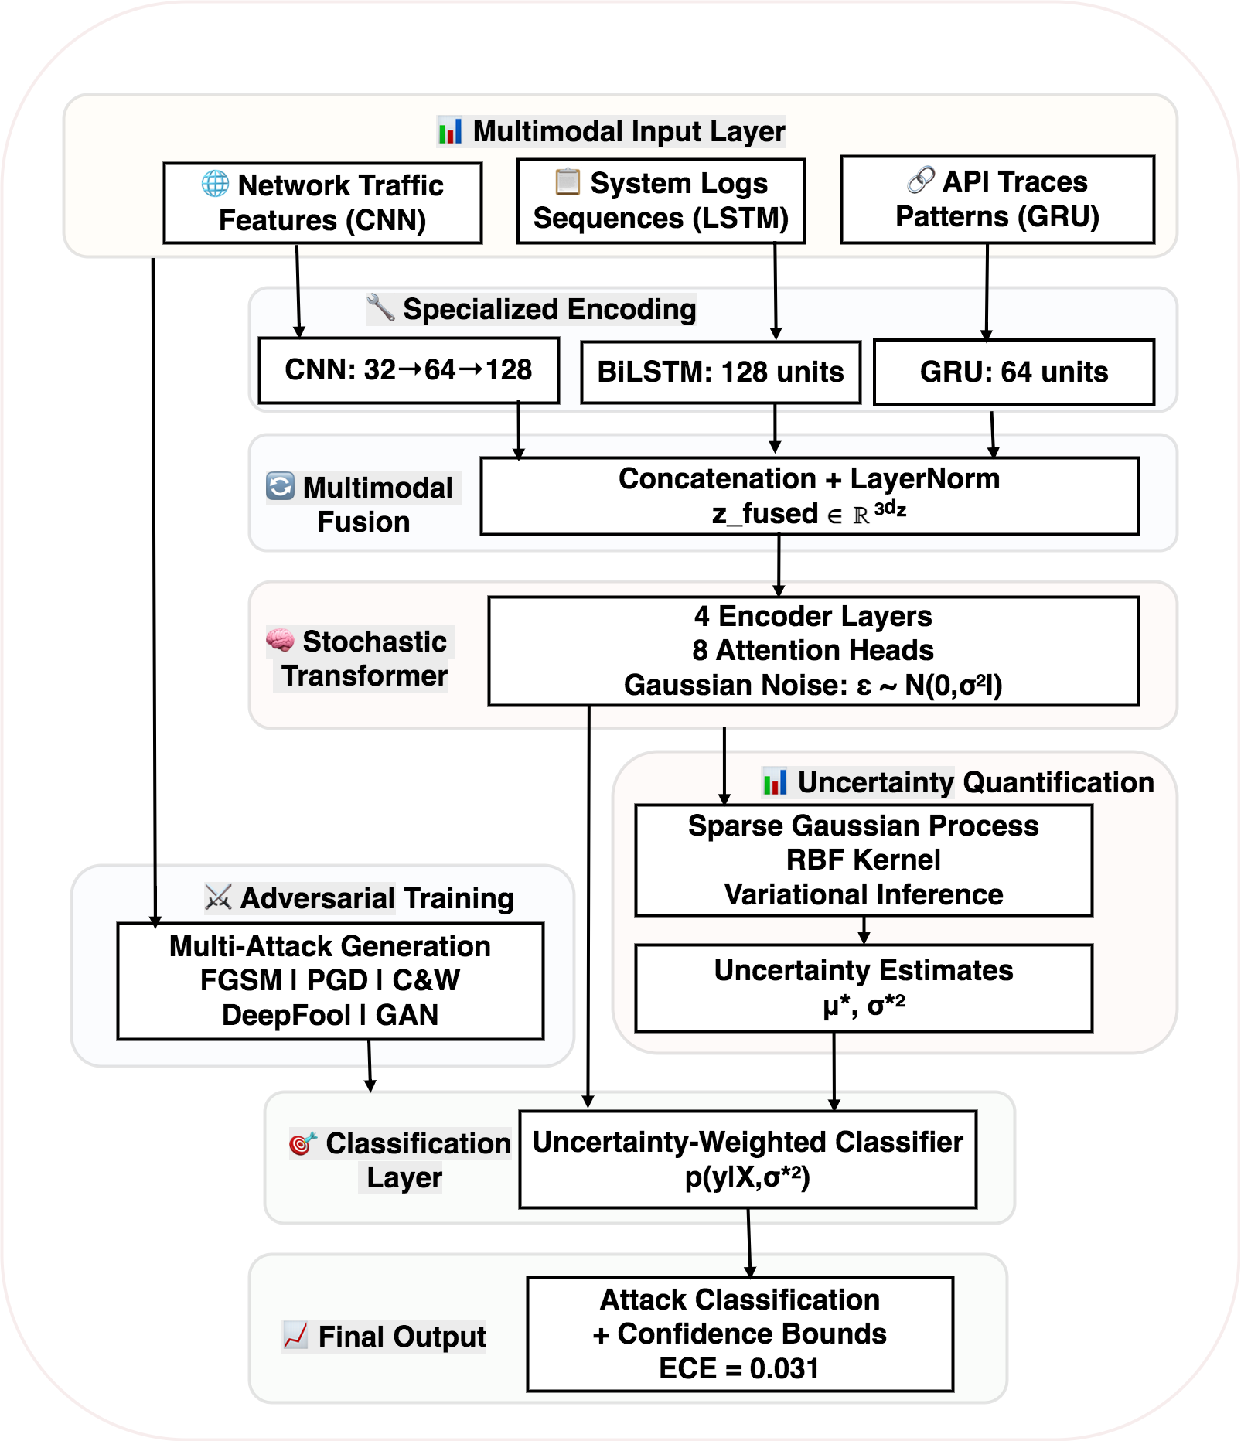
\includegraphics[width=0.95\linewidth]{figures/fig_stochastic_transformer_architecture.pdf}
\end{columns}
\end{frame}

% ============================================================
% Slide 38: M7
% ============================================================
\begin{frame}{M7: Единая система сертификации Hybrid IDPS}
\scriptsize
\textbf{Теоретико-игровая робастность:} равновесия Штакельберга
+ мультипликативные веса онлайн-обучения
\[
R(T)\le 2\sqrt{T\log|\mathcal{C}|}\ \Rightarrow\ R(T)/T\to 0
\]
{\scriptsize $R(T)$: кумулятивный регрет после $T$ раундов;
$\mathcal{C}$: мн-во конфигураций защитника}\smallskip

\textbf{Связанная оптимизация:} все 7~моделей интегрированы
через регуляризацию согласованности
\[
\mathcal{L}_{\text{unified}}=\underbrace{\sum_{i=1}^{7}\lambda_i\mathcal{L}_i}_{\text{потери методов}}
+\underbrace{\sum_{i<j}\lambda_{ij}[\mathrm{KL}(p_i\|p_j)+\|z_i-z_j\|^2]}_{\text{попарная согласованность}}
\]
{\scriptsize $\lambda_i$: вес метода; $\mathcal{L}_i$: потери метода~$i$;
KL: согл.\ предсказаний; $\|z_i-z_j\|^2$: выравн.\ вложений}\smallskip

\textbf{Теорема (Сходимость):}
$\displaystyle \|\nabla\mathcal{L}_{\text{unified}}(\theta_T)\|^2\le\frac{2(\mathcal{L}_0-\mathcal{L}^*)}{\eta_{\min}T}$\smallskip

\begin{alertblock}{}
\scriptsize \textbf{6 теорем:} сходимость CT-TGNN, сертификат
Липшица, византийская сходимость, PAC-Байес, граница регрета,
единая сходимость семейства M1--M7 в составе Hybrid IDPS.
\end{alertblock}
\end{frame}

% ============================================================
% Slide 39: Chapter 3 divider
% ============================================================
\begin{frame}{3: Адаптация Hybrid IDPS к системам обнаружения и предотвращения сетевых вторжений}
\vspace{1.5cm}
\begin{center}
{\Large\bn{Адаптация и согласование с сетевыми NIDPS}}\\[1cm]

Предметно-ориентированная глава: терминология,\\
конвейер данные$\to$граф, таксономия из 34~классов,\\
инженерия 83~признаков, гиперпараметры,\\
реализации методов M1--M7 с 8~архитектурными схемами\\[0.6cm]

\textit{Все формальные результаты Главы 2 \textbf{предметно-независимы}.\\
Глава 3 инстанцирует их в NIDPS-секторе как\\
основной инстанции Hybrid IDPS.}
\end{center}
\end{frame}

% ============================================================
% Slide 40: Конвейер данные -> граф
% ============================================================
\begin{frame}{Конвейер преобразования данных в граф}
\begin{columns}[T,onlytextwidth]
\column{0.55\textwidth}
\scriptsize
\textbf{Сырой трафик $\to$ Граф Hybrid IDPS:}
\begin{itemize}\setlength\itemsep{0pt}
\item \bn{Узлы:} IP-адреса (хосты).
Признак: 12-мерная статистика хоста
\item \bn{Рёбра:} сетевые потоки.
Признак: 83-мерный вектор потока
\item \bn{Темпоральность:} потоки истекают через 120~с
\end{itemize}
\medskip
\textbf{Многоуровневость (TripleE):}
\begin{itemize}\setlength\itemsep{0pt}
\item Граф сервисов $\mathcal{G}_s$: API-вызовы
\item Граф трассировок $\mathcal{G}_r$: цепочки запросов
\item Граф хостов $\mathcal{G}_n$: потоки трафика
\end{itemize}
\medskip
\[
\tilde{f}_j=\frac{f_j-\mu_j}{\sigma_j+\varepsilon}
\]
{\scriptsize z-нормализация для каждого признака}

\column{0.45\textwidth}
\textbf{83 инженерных признака:}\\[2pt]
\scriptsize
\begin{tabular}{lr}
\toprule
Категория & Кол-во \\
\midrule
Статистика потоков & 22 \\
Распределения IAT & 18 \\
Флаговые индикаторы & 15 \\
Статистика полезной нагрузки & 16 \\
Производные отношения & 12 \\
\midrule
\textbf{Всего} & \textbf{83} \\
\bottomrule
\end{tabular}
\end{columns}
\end{frame}

% ============================================================
% Slide 41: Таксономия 34 класса
% ============================================================
\begin{frame}{Таксономия классификации Hybrid IDPS: 34 класса}
\scriptsize
\begin{tabular}{p{2.6cm}p{9.4cm}}
\toprule
\textbf{Категория (кол-во)} & \textbf{Классы атак} \\
\midrule
DDoS (8) & TCP, UDP, ICMP, HTTP, SYN Flood, DNS Amp, SSDP, NTP Amp \\
DoS (5) & GoldenEye, Hulk, Slowhttptest, Slowloris, HeartBeat \\
Разведка (4) & PortScan, Nmap, Service Probe, OS Fingerprint \\
Перебор (4) & FTP-Patator, SSH-Patator, Web Login, RDP \\
Веб-атаки (4) & XSS, SQL Injection, Command Injection, Directory Traversal \\
ВПО (5) & Mirai, Botnet, Trojan, Ransomware, Cryptomining \\
Продвинутые (3) & Infiltration, Heartbleed, Spoofing \\
Легитимный (1) & Нормальный трафик \\
\bottomrule
\end{tabular}
\medskip

\begin{alertblock}{}
\small\textbf{Расширяемость:} новые классы атак через
CyberSecLLM zero-shot~+ TripleE-TGNN инкрементальное обучение
без переобучения остального контура Hybrid IDPS.
\end{alertblock}
\end{frame}

% ============================================================
% Slide 42: Гиперпараметры
% ============================================================
\begin{frame}{Реализации методов и гиперпараметры}
\small
\begin{tabular}{p{2.5cm}p{2.5cm}p{2.5cm}p{4.0cm}}
\toprule
\textbf{Метод} & \textbf{Параметр} & \textbf{Значение} & \textbf{Обоснование} \\
\midrule
M1: CT-TGNN & Пост.\ врем. & $1/60/3600$\,с & Пакет/сессия/кампания \\
M2: FedLLM-API & Бюджет ДП & $(0{,}85,10^{-5})$ & Строгая приватность \\
M3: TripleE & EWC $\lambda$ & 0,5 & Защита от забывания \\
M4: MambaShield & Ядро & 1024 & Охват последоват. \\
M5: Сточ.\ трансф. & Выборки МК & 50 & Качество неопред. \\
M7: Сертификация & MWU $\eta$ & $\sqrt{\log|\mathcal{C}|/T}$ & Оптимальный регрет \\
\bottomrule
\end{tabular}
\medskip

\begin{block}{}
\small Все значения подобраны поиском по сетке на
валидационном наборе CIC-IoT-2023.\\[2pt]
\textbf{Реализация:} PyTorch 2.1, CUDA 12.1, AdamW
($\eta=2\times10^{-4}$).
\end{block}
\end{frame}

% ============================================================
% Slide 43: Интегрированный конвейер
% ============================================================
\begin{frame}{Интегрированный конвейер обнаружения Hybrid IDPS}
\centering
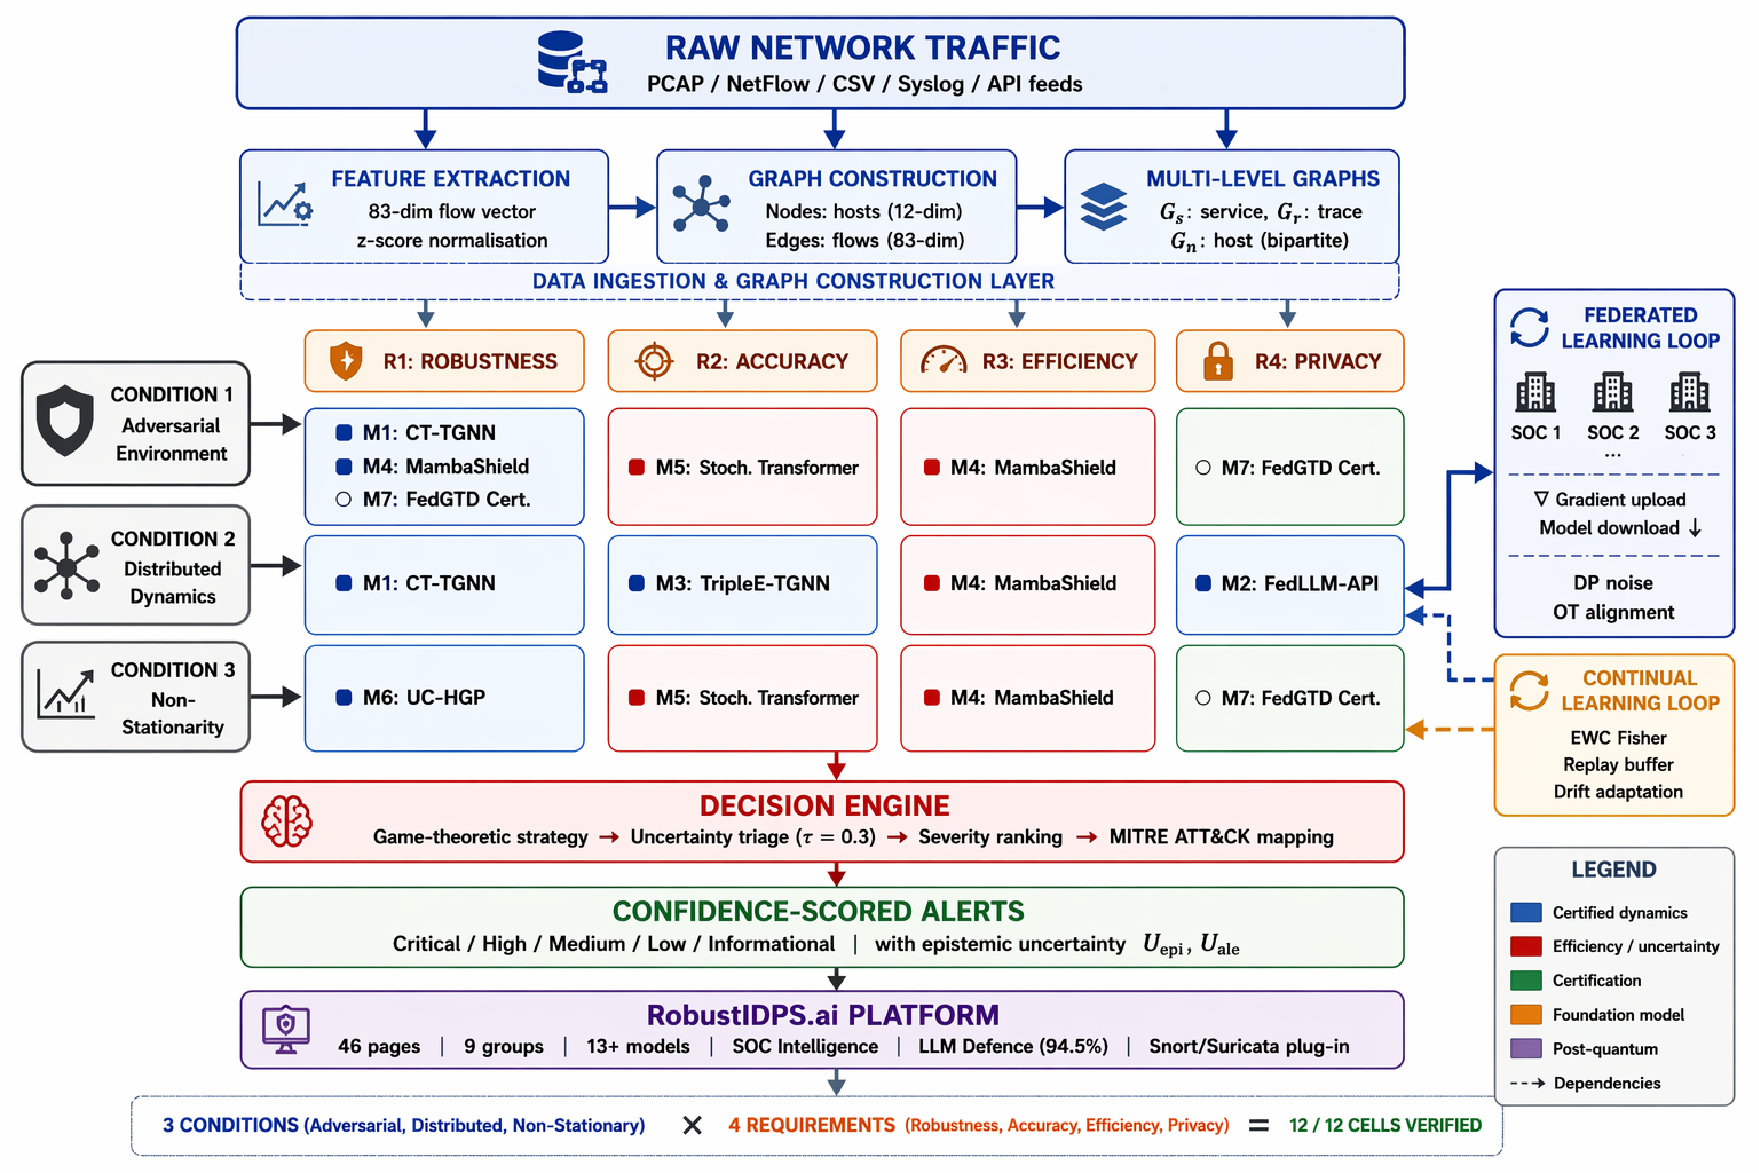
\includegraphics[width=0.95\linewidth]{figures/Main_arch_v1b.pdf}\\[4pt]
{\scriptsize Сырой трафик $\to$ извлечение 83~признаков $\to$
M1--M7 параллельно $\to$ теоретико-игровой механизм принятия
решений $\to$ оповещения с оценкой уверенности.
Развёртывается как \hl{плагин для Snort/Suricata} в составе
коммерческого Hybrid IDPS контура.}
\end{frame}

% ============================================================
% Slide 44: Chapter 4 divider
% ============================================================
\begin{frame}{4: Экспериментальные результаты и валидация}
\vspace{1.5cm}
\begin{center}
{\Large\bn{6 наборов данных, 84,2~млн образцов, 23 метрики}}\\[1cm]

11 таблиц~|~8 рисунков\\[0.4cm]

Результаты по моделям M1--M7, базовые линии, абляция,\\
состязательная робастность, кросс-доменный перенос,\\
обнаружение MA-PQC, кросс-сектора Hybrid IDPS\\[0.6cm]

\textit{Превосходство над лучшими базовыми методами\\
на \textbf{2,9--5,6 п.\,п.} по всем наборам данных}
\end{center}
\end{frame}

% ============================================================
% Slide 45: Результаты бенчмарков
% ============================================================
\begin{frame}{Результаты бенчмарков Hybrid IDPS: единая система}
\begin{columns}[T,onlytextwidth]
\column{0.42\textwidth}
\small
\begin{tabular}{lccc}
\toprule
Набор данных & Точн. & Базов. & $\Delta$ \\
\midrule
CIC-IoT (46,6M) & 94,7 & 91,8 & +2,9 \\
CICIDS (16,2M) & 93,9 & 89,7 & +4,2 \\
UNSW (2,5M) & 93,8 & 88,2 & +5,6 \\
MS GUIDE (13,7M) & 92,1 & 87,5 & +4,6 \\
Container (3,2M) & 91,5 & 86,9 & +4,6 \\
Edge-IIoT (2,0M) & 89,8 & 84,3 & +5,5 \\
\bottomrule
\end{tabular}\smallskip

\begin{alertblock}{}
\small\hl{+2,9 до +5,6 п.\,п.}\\
улучшение на всех 6 наборах данных (84,2~млн образцов)
\end{alertblock}

\column{0.58\textwidth}
\centering
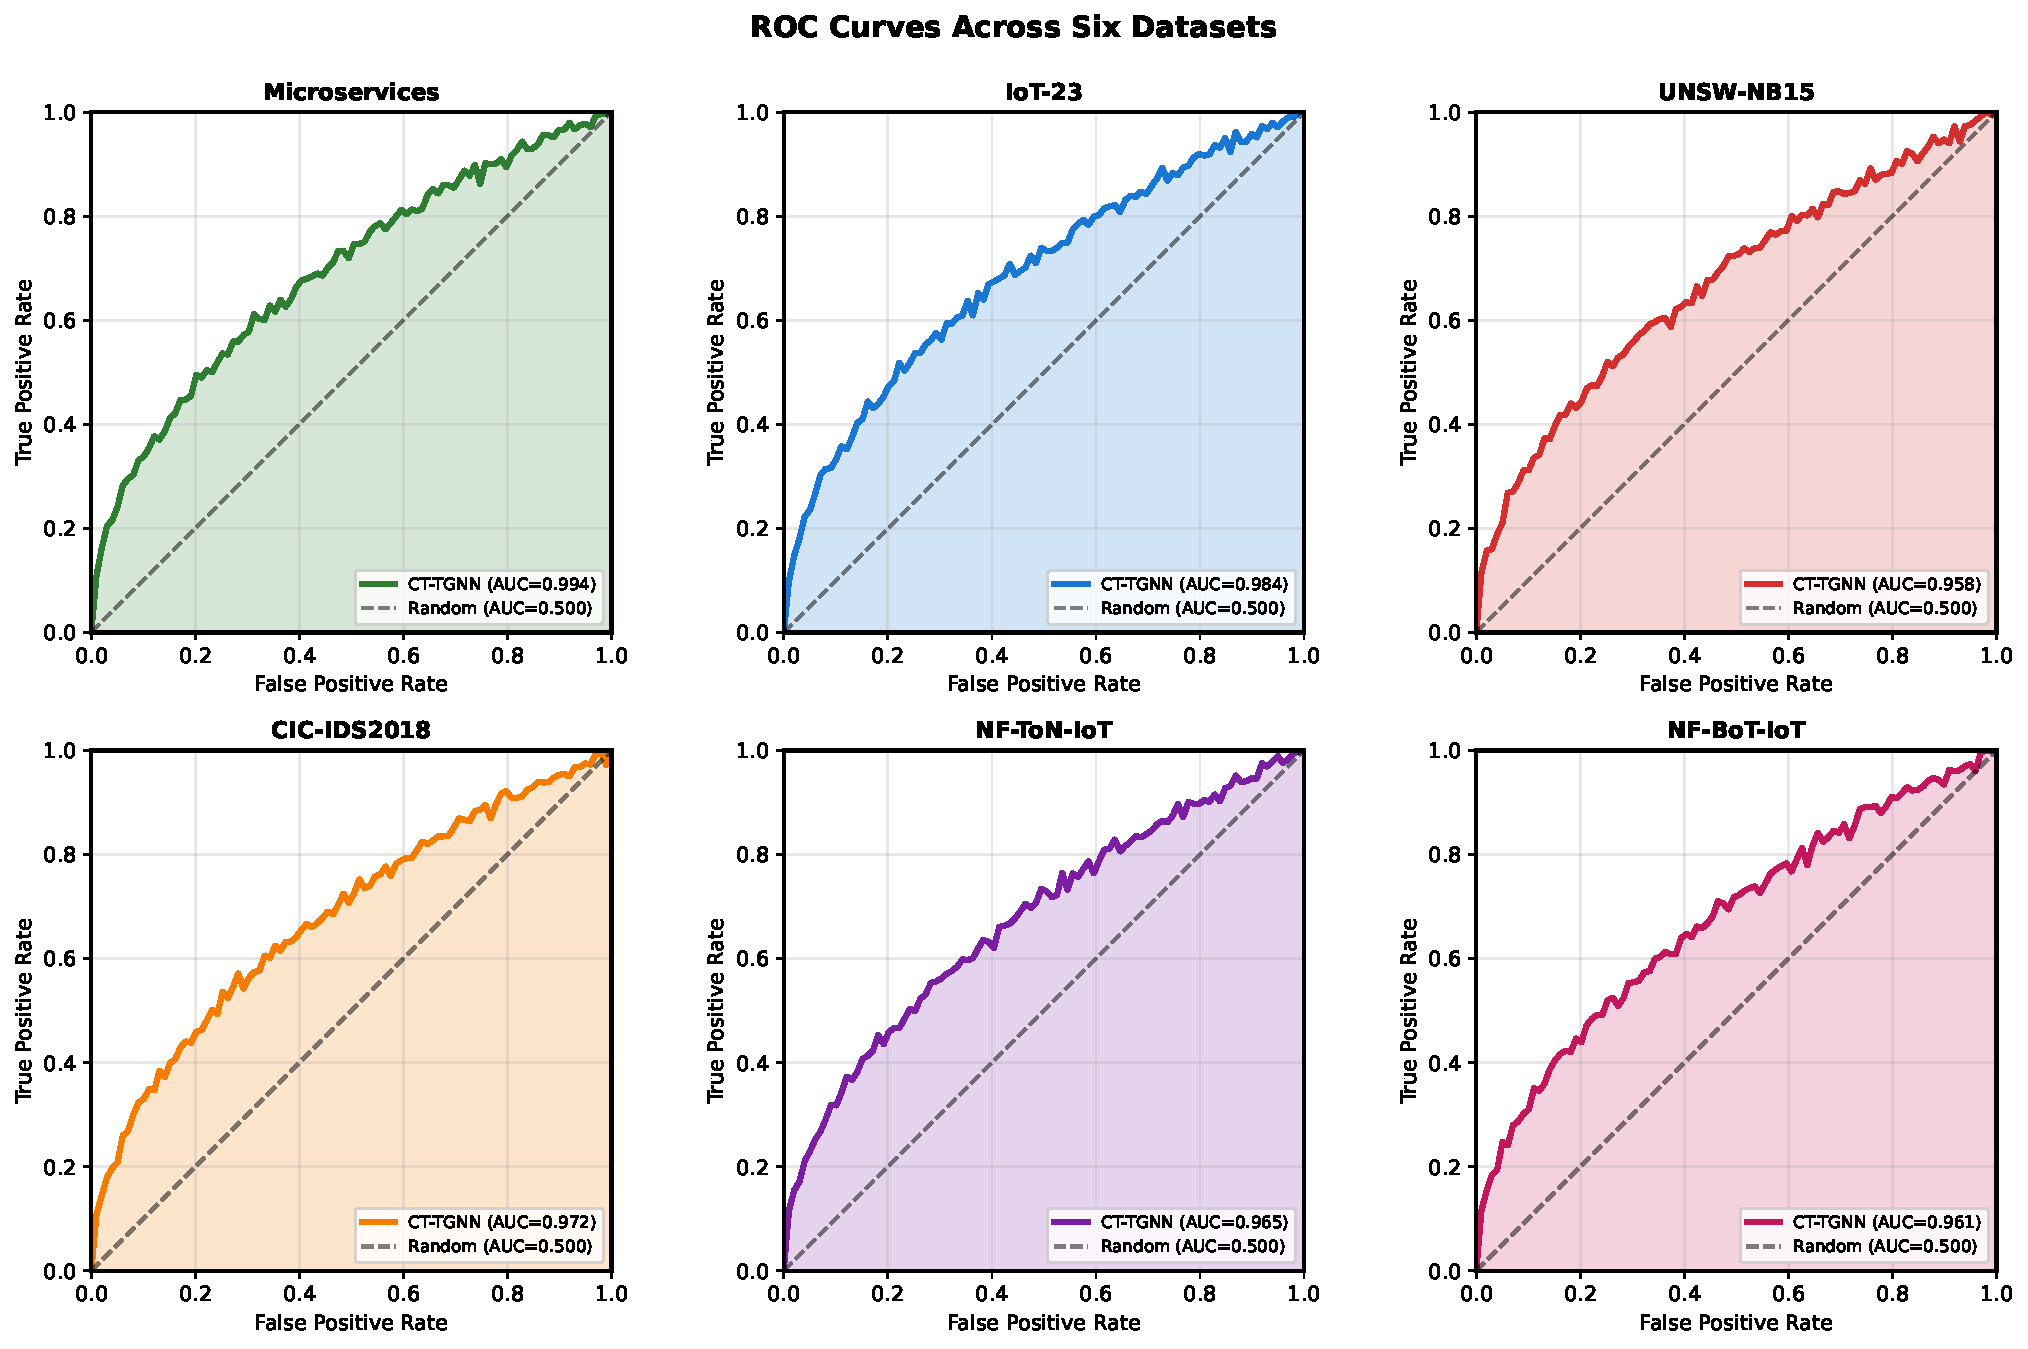
\includegraphics[width=0.95\linewidth]{figures/Figure6_ROC_Generalization.pdf}\\[2pt]
{\scriptsize ROC-кривые и кросс-доменное обобщение Hybrid IDPS}
\end{columns}
\end{frame}

% ============================================================
% Slide 46: Основные результаты по методам
% ============================================================
\begin{frame}{Основные результаты по моделям Hybrid IDPS}
\begin{columns}[T,onlytextwidth]
\column{0.50\textwidth}
\small
\textbf{CT-TGNN:} 98,3\% точн., 47~мс задержка\\
\textbf{SDE-TGNN:} 99,0\% F1, 76,2\% сертифиц.\ при $R{=}0{,}25$\\
\textbf{FedLLM-API:} 87,1\% при 40\% византийских\\
\textbf{TripleE-TGNN:} 96,8\% многоуровн.\\
\textbf{MambaShield:} 91,4\% при 25\% отравления\\
\textbf{Задержка:} \hl{0,5~мс/поток} (MambaShield)

\column{0.50\textwidth}
\small
\textbf{M5/M6:} ECE 0,078 ($-$59\% отн.\ детерминист.)\\
43\% снижение нагрузки аналитиков (P5)\\
\textbf{M7:} 94,7\% против адаптивных противников\\
$R(T)\le 2\sqrt{T\log|\mathcal{C}|}$ подтверждено\\
\textbf{CyberSecLLM:} 89,1\% zero-shot\\
($+$20,5~п.\,п.\ над GPT-4)\\
Миллион токенов за 2,3~с
\end{columns}
\medskip
\begin{block}{}
\small\textbf{Кросс-доменный перенос Hybrid IDPS:} 90,5\%~F1
без дообучения (речь LibriSpeech 94,2\%, здравоохранение
MIMIC-III/eICU 89,7\%).
\end{block}
\end{frame}

% ============================================================
% Slide 47: Абляция и состязательная робастность
% ============================================================
\begin{frame}{Абляция и состязательная робастность Hybrid IDPS}
\begin{columns}[T,onlytextwidth]
\column{0.48\textwidth}
\textbf{Основные результаты абляции:}\\
\scriptsize
\begin{tabular}{lc}
\toprule
Удалённый компонент & $\Delta$ (п.\,п.)\\
\midrule
Ветвь LLM (F1) & $-$53,4 \\
Визант.\ $\to$ FedAvg & $-$21,4 \\
ОТ выравнивание & $-$15,8 \\
Прогресс.\ дистилляция & $-$9,7 \\
Теор.-игр.\ равновесие & $-$7,1 \\
НВ ОДУ $\to$ дискр.\ RNN & $-$6,8 \\
\bottomrule
\end{tabular}\medskip
\begin{block}{}
\scriptsize Каждый компонент M1--M7 вносит измеримый вклад в
единый контур Hybrid IDPS.
\end{block}

\column{0.48\textwidth}
\textbf{Состязательная робастность (6 атак):}\\
\scriptsize
\begin{tabular}{lcc}
\toprule
Атака & Чист. & Робаст.\ (AT) \\
\midrule
FGSM & 97,8 & 93,1 \\
PGD-40 & 97,8 & 89,6 \\
C\&W & 97,8 & 85,2 \\
DeepFool & 97,8 & 90,8 \\
Gaussian & 97,8 & 95,3 \\
Label Masking & 97,8 & 93,7 \\
\bottomrule
\end{tabular}\medskip
\begin{block}{}
\scriptsize Макс.\ деградация: 12,6~п.\,п.\ (C\&W).
\textbf{Сертифицировано:} 76,2\% при $R{=}0{,}25$.
\end{block}
\end{columns}
\end{frame}

% ============================================================
% Slide 48: MA-PQC
% ============================================================
\begin{frame}{Результаты Multi-Agent PQC-IDS для Hybrid IDPS}
\begin{columns}[T,onlytextwidth]
\column{0.48\textwidth}
\textbf{Основные достижения:}
\begin{itemize}\setlength\itemsep{0pt}
\item \textbf{Основа MambaShield:} 96,7\% точн.\ при ускорении в~7,3$\times$
\item \textbf{Структурированная FIM:} 38\% снижение забывания
\item \textbf{Координация MA-CPO:} 96,1\% нейтрализация,
\hl{ноль нарушений ограничений}, 34\% снижение задержки
\end{itemize}
\smallskip
При C\&W через миграцию PQC: только 2,5~п.\,п.\ деградации
против 25,5~п.\,п.\ при дообучении.

\column{0.52\textwidth}
\textbf{Обнаружение по семействам пост-квантовых протоколов:}\\
\scriptsize
\begin{tabular}{llc}
\toprule
Протокол & Атака & Точн. \\
\midrule
Решётки (Kyber) & Атака на кэш & 97,3 \\
Решётки (Kyber) & Инъекция ошибок & 94,8 \\
Коды (McEliece) & Декод.\ инф.\ мн. & 95,1 \\
Хэш (SPHINCS+) & Исчерп.\ ресурсов & 94,7 \\
Кросс-протокол & Понижение & 98,3 \\
\midrule
\textbf{Общий} & & \textbf{96,2} \\
\bottomrule
\end{tabular}\smallskip

\scriptsize 4 кооперативных агента: Аналитик трафика,
Специалист PQC, Детектор аномалий, Координатор.
\end{columns}
\end{frame}

% ============================================================
% Slide 49: Chapter 5 divider
% ============================================================
\begin{frame}{5: Программная платформа RobustIDPS.ai}
\vspace{1.5cm}
\begin{center}
{\Large\bn{Реализация: \hl{51-страничное} PWA,\\
\hl{10~функциональных групп}, \hl{17~моделей}}}\\[1cm]

DOI: 10.5281/zenodo.19129512\\[4pt]
\texttt{https://robustidps.ai}\\
\texttt{github.com/rogerpanel/robustidps.ai}\\[1cm]

\textit{Промышленный Hybrid IDPS:\\
4-уровневая защита LLM~|~Multi-Agent PQC-IDS~|~Плагин Snort/Suricata}
\end{center}
\end{frame}

% ============================================================
% Slide 50: Структура и возможности платформы
% ============================================================
\begin{frame}{Общая структура и возможности платформы Hybrid IDPS}
\begin{columns}[T,onlytextwidth]
\column{0.50\textwidth}
\small
\textbf{Технологический стек:}
\begin{itemize}\setlength\itemsep{0pt}
\item React~18 PWA фронтенд
\item Flask/Python 3.11+ бэкенд
\item PostgreSQL 16 + Redis 7
\item Развёртывание Docker Compose
\item 60+ REST API эндпоинтов
\end{itemize}
\smallskip
\textbf{Целевые пользователи:}
\begin{itemize}\setlength\itemsep{0pt}
\item SOC-аналитики (уровни 1--3)
\item Инженеры кибербезопасности
\item Исследователи MLSecOps
\item Разработчики ИИ
\item Научные исследователи
\end{itemize}

\column{0.50\textwidth}
\small
\begin{tabular}{lc}
\toprule
Функциональная группа & Стр. \\
\midrule
1. AI Command Center & 6 \\
2. AI Active Defence & 5 \\
3. SOC Intelligence Suite & 6 \\
4. LLM Attack Surface & 5 \\
5. MLSecOps Standards & 3 \\
6. AI Security \& Govern. & 4 \\
7. AI Novel Methods & 6 \\
8. AI Data \& Models & 3 \\
9. Multi-Agent PQC-IDS & 5 \\
10. System Administration & 8 \\
\midrule
\textbf{Всего} & \hl{\textbf{51}} \\
\bottomrule
\end{tabular}
\end{columns}
\end{frame}

% ============================================================
% Slide 51: SOC + LLM defence
% ============================================================
\begin{frame}{SOC-аналитика + Защита LLM Hybrid IDPS}
\begin{columns}[T,onlytextwidth]
\column{0.50\textwidth}
\small
\textbf{Пакет SOC-аналитики (6 страниц):}
\begin{itemize}\setlength\itemsep{0pt}
\item Агентное автоматическое расследование
\item Поиск угроз на естественном языке
\item Автоматизированные отчёты об инцидентах
\item Генератор правил СОВ (Snort/Suricata)
\item Маппер уязвимостей CVE
\end{itemize}
\smallskip
\begin{block}{}
\scriptsize\textbf{Пользовательское исследование:}
\hl{34\% снижение времени сортировки} ($4,7\to3,1$ мин/оповещение).
\end{block}

\column{0.50\textwidth}
\textbf{Защита LLM (5 страниц):}\\
\small
\begin{tabular}{lc}
\toprule
Модуль & Обнар.\ \% \\
\midrule
Инъекция промптов & 96,3 \\
Джейлбрейк & 95,1 \\
Отравление RAG & 93,7 \\
Мультиагентные & 91,8 \\
Отравление данных & 95,6 \\
\midrule
\textbf{Общий} & \hl{\textbf{94,5}} \\
\bottomrule
\end{tabular}\smallskip

\scriptsize \textbf{4 LLM-бэкенда протестированы:}
Claude, GPT-4o, Gemini, DeepSeek.
\end{columns}
\end{frame}

% ============================================================
% Slide 52: Модели платформы и сравнение
% ============================================================
\begin{frame}{Модели платформы и сравнение Hybrid IDPS}
\small
\begin{tabular}{lccc}
\toprule
Модель & Точн.\ \% & ECE & Задержка \\
\midrule
SurrogateIDS (7 ветвей) & 97,8 & 0,031 & 0,8~мс \\
CyberSecLLM & 97,1 & 0,025 & 6,8~мс \\
CT-TGNN (M1) & 96,2 & 0,049 & 1,2~мс \\
MambaShield (M4) & 95,9 & 0,042 & \hl{0,5~мс} \\
Multi-Agent PQC-IDS & 94,3 & 0,044 & 1,5~мс \\
\bottomrule
\end{tabular}
\medskip
\begin{block}{Отличия от коммерческих платформ}
\small
Открытый код~\checkmark~|~Мультипровайдерный LLM~\checkmark~|~Состязательное тестирование~\checkmark\\
Постквантовая СОВ~\checkmark~|~NIST AI RMF~\checkmark~|~Плагин Snort/Suricata~\checkmark
\end{block}
\smallskip
\begin{alertblock}{}
\small RobustIDPS.ai~--- единственный известный Hybrid IDPS
с одновременно \hl{17~моделями}, \hl{10~функциональными
группами}, 4~LLM-бэкендами, MA-PQC и интеграцией со Snort/Suricata.
\end{alertblock}
\end{frame}

% ============================================================
% Slide 53-56: Screenshots
% ============================================================
\begin{frame}{Скриншоты платформы Hybrid IDPS (1/4): Панель управления}
\centering
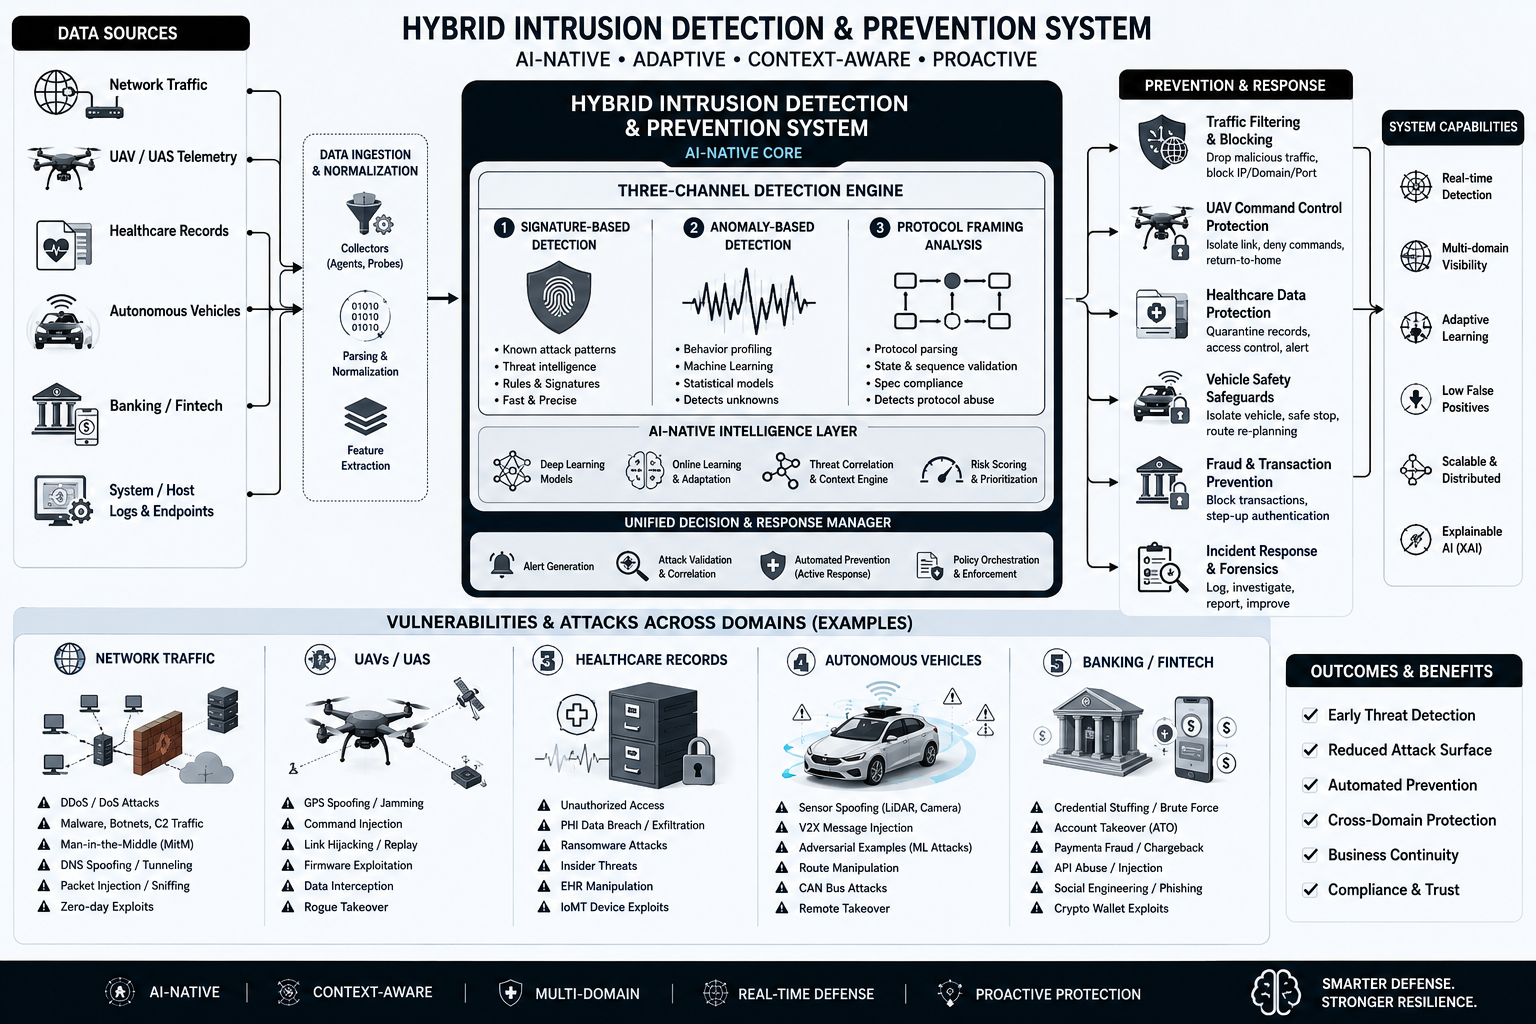
\includegraphics[width=0.85\linewidth]{figures/fig_nidps_v1.png}\\[2pt]
{\scriptsize Панель управления RobustIDPS.ai: обзор контура
Hybrid IDPS с обучаемыми компонентами M1--M7}
\end{frame}

\begin{frame}{Скриншоты платформы Hybrid IDPS (2/4): Модели}
\centering
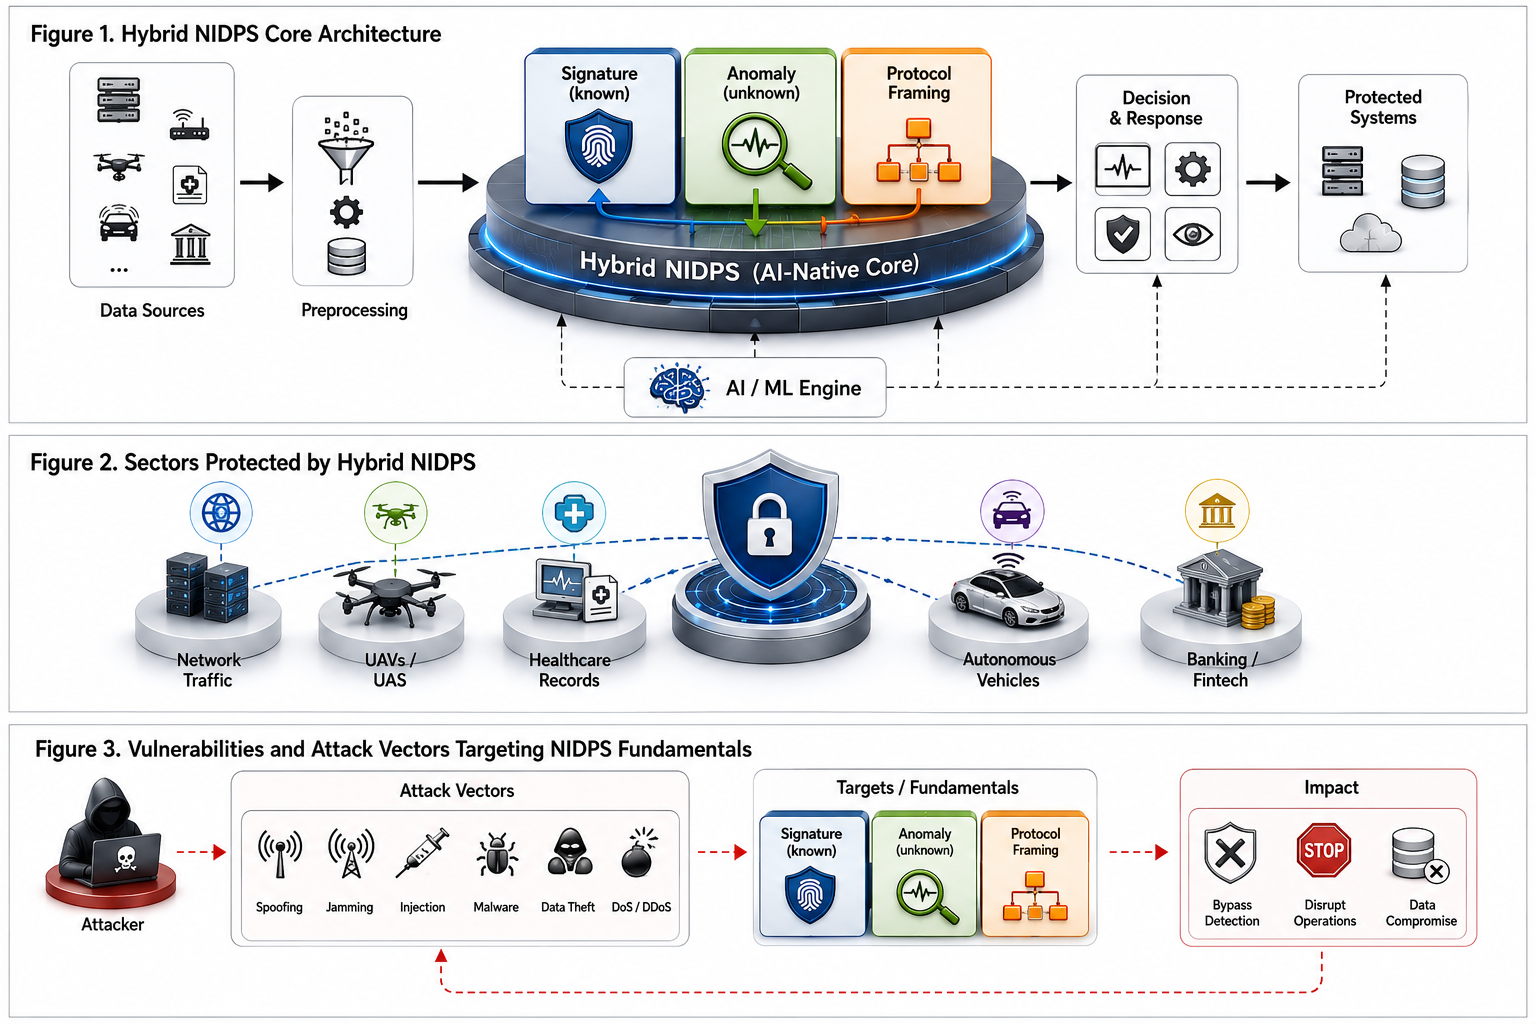
\includegraphics[width=0.85\linewidth]{figures/fig_nidps_v2.png}\\[2pt]
{\scriptsize Каталог моделей RobustIDPS.ai (17~интегрированных):
все 7~оригинальных M1--M7 плюс CyberSecLLM, MA-PQC и
дополнительные конфигурации}
\end{frame}

\begin{frame}{Скриншоты платформы Hybrid IDPS (3/4): SOC-аналитика}
\centering
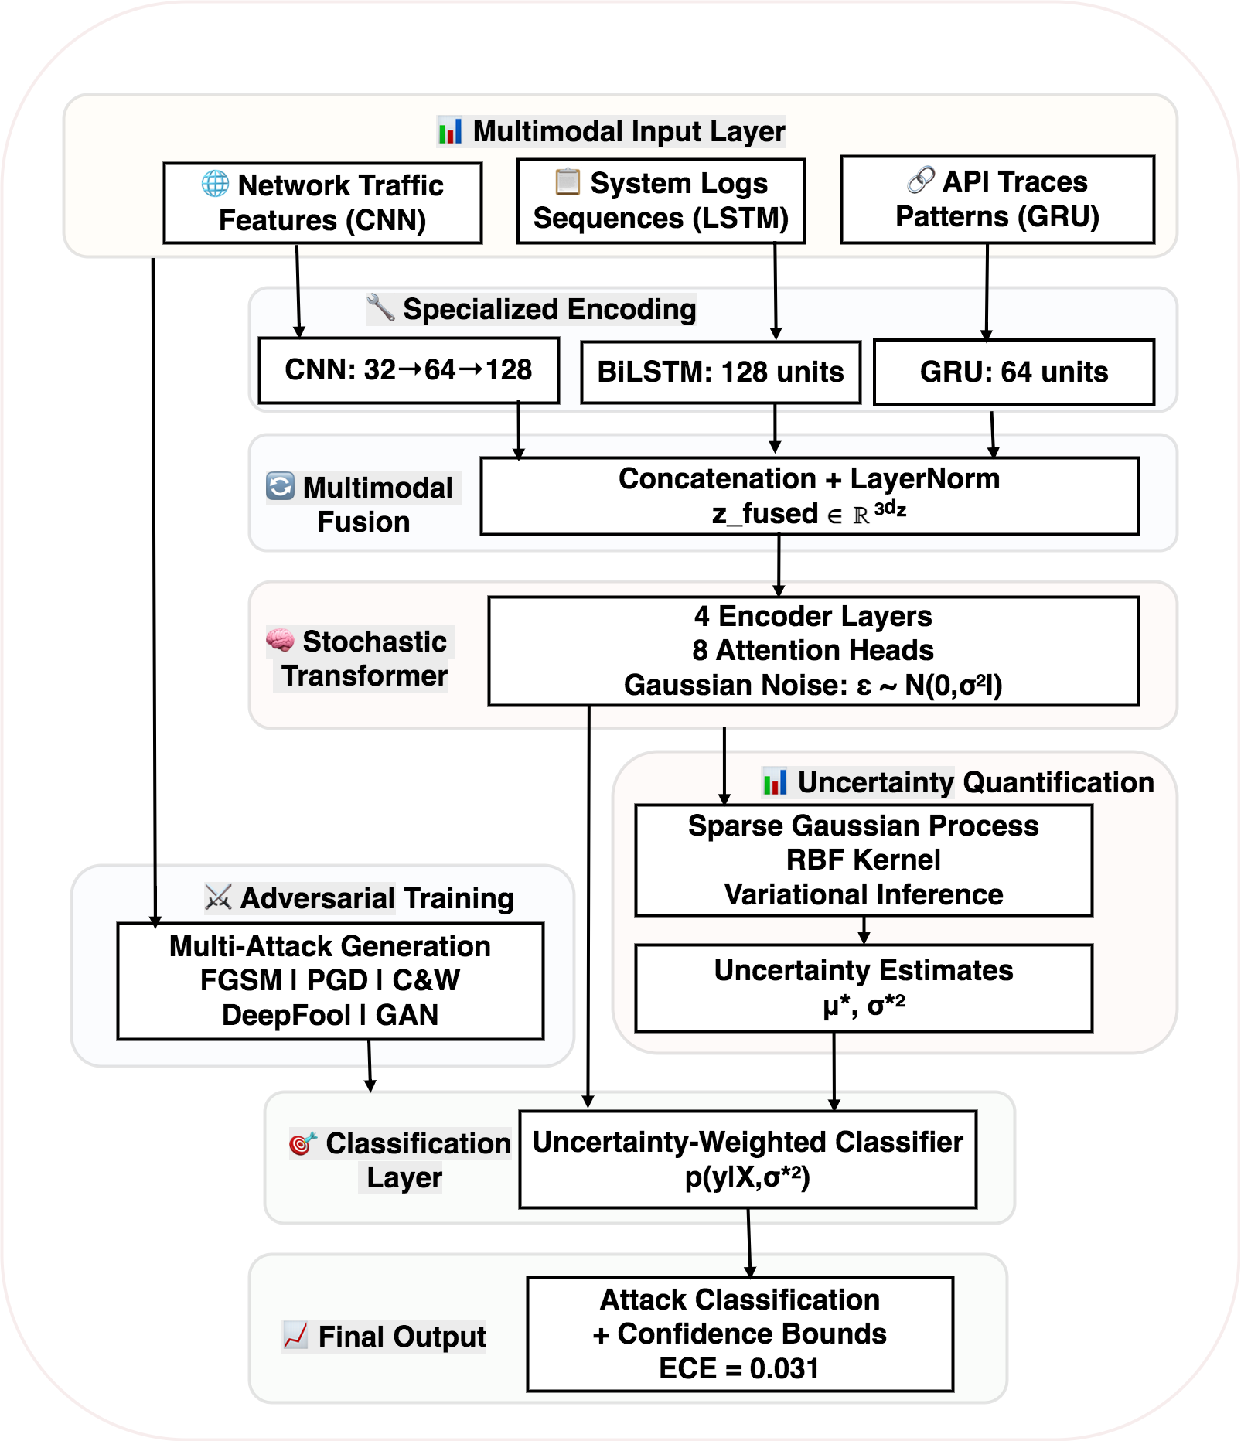
\includegraphics[width=0.85\linewidth]{figures/fig_stochastic_transformer_architecture.pdf}\\[2pt]
{\scriptsize SOC Copilot RobustIDPS.ai: автоматическое
расследование инцидентов с использованием Claude, GPT-4o,
Gemini, DeepSeek и оценкой эпистемической неопределённости
от UC-HGP}
\end{frame}

\begin{frame}{Скриншоты платформы Hybrid IDPS (4/4): MA-PQC}
\centering
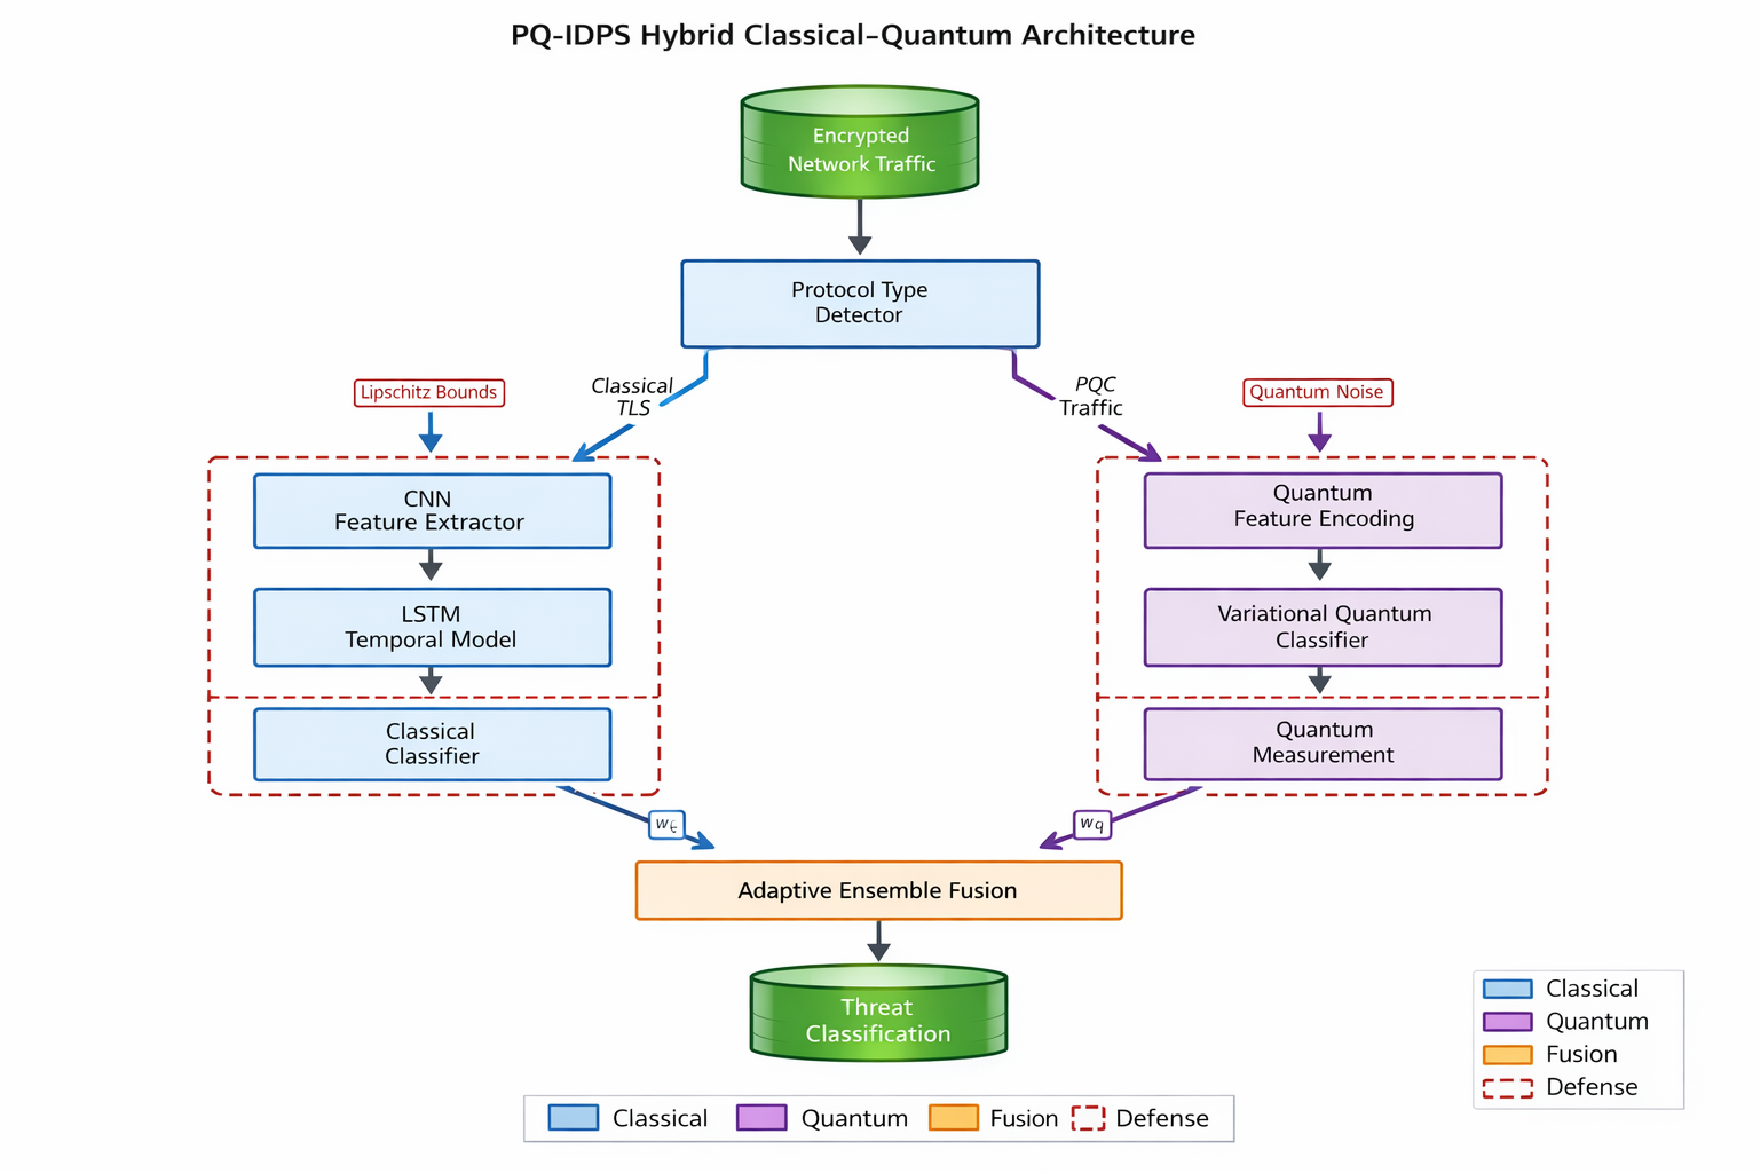
\includegraphics[width=0.85\linewidth]{figures/fig_pq_idps_architecture.pdf}\\[2pt]
{\scriptsize Модуль Multi-Agent PQC-IDS: 4~кооперативных
агента для обнаружения атак на пост-квантовые протоколы~---
расширение Hybrid IDPS на форвард-совместимое детектирование}
\end{frame}

% ============================================================
% Slide 57: Заключение - основные результаты
% ============================================================
\begin{frame}{Заключение: основные результаты}
\scriptsize
\begin{enumerate}\setlength\itemsep{1pt}
\item \bn{Единое описание Hybrid IDPS:} кортеж $\mathcal{H}$ и
6~свойств P1--P6, матрица $3\times4$
\item \bn{CT-TGNN/SDE-TGNN:} \emph{Первая} сертифицированная
динамика НВ-графов в Hybrid IDPS~--- 99,0\% F1, 76,2\% сертифиц.,
90,5\% перенос
\item \bn{FedLLM-API:} \emph{Оригинальный} византийско-устойчивый
федеративный~--- 87,1\% при 40\% повреждений, ($\varepsilon{=}0{,}85$) ДП
\item \bn{TripleE-TGNN:} \emph{Новые} многоуровневые вложения~---
96,8\% с защитой от забывания
\item \bn{MambaShield:} \emph{Новая} SSM $\mathcal{O}(L\log L)$~---
91,4\% при 25\% отравления, 0,5~мс задержка
\item \bn{Сточ.\ трансф.+UC-HGP:} \emph{Первая} интегрированная
неопределённость в Hybrid IDPS~--- ECE 0,078, 43\% снижение нагрузки
\item \bn{M7 сертификация:} \emph{Оригинальная} теоретико-игровая~---
94,7\% против адаптивных противников
\item \bn{CyberSecLLM:} \emph{Новая} фундаментальная модель~---
89,1\% zero-shot ($+$20,5~п.\,п.\ над GPT-4)
\item \bn{Предметная адаптация:} таксономия 34 классов, конвейер
83 признаков, плагин Snort/Suricata
\item \bn{Валидация:} 84,2~млн образцов, 6 наборов данных,
23 метрики, все 12 ячеек матрицы подтверждены
\item \bn{RobustIDPS.ai:} \hl{51-страничная} платформа,
\hl{17~моделей}, 94,5\% защита LLM, 4 акта внедрения
\end{enumerate}
\end{frame}

% ============================================================
% Slide 58: Результаты задач (single big figure)
% ============================================================
\begin{frame}{Результаты решения задач исследовательского пространства}
\centering
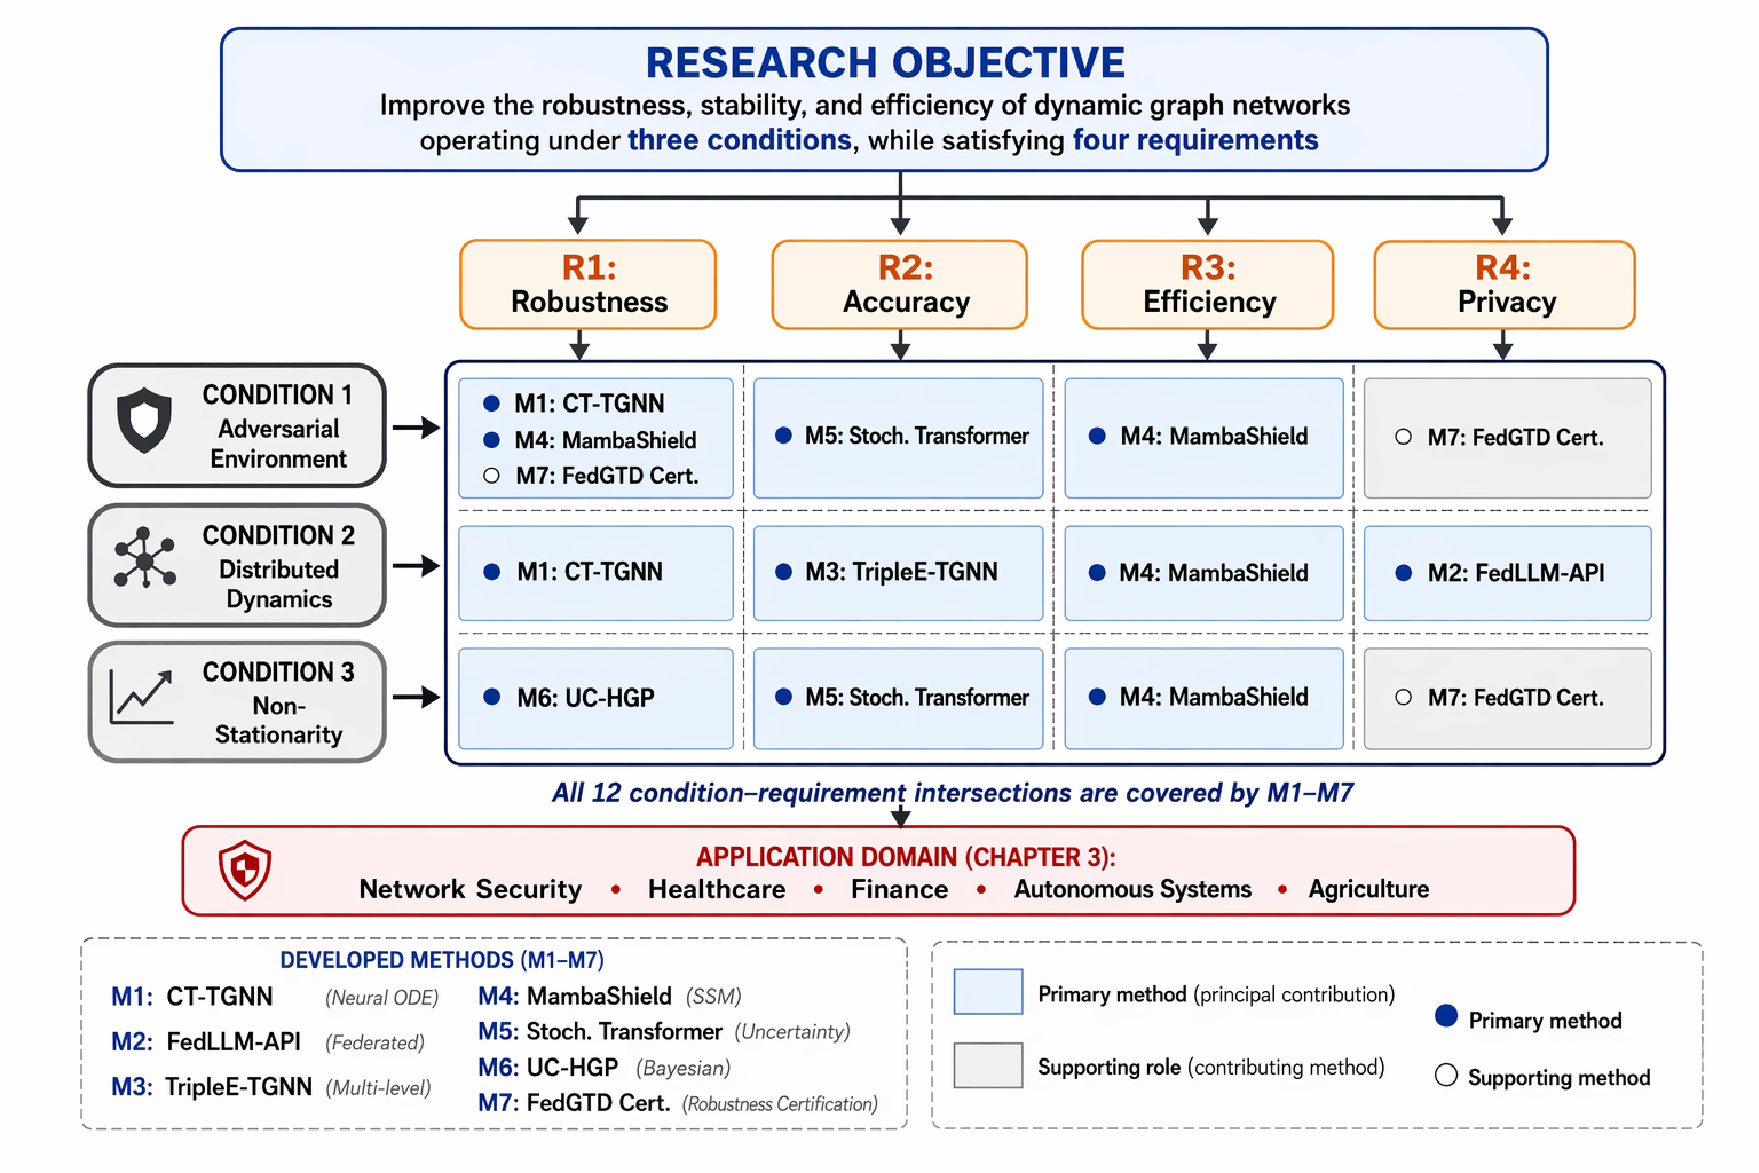
\includegraphics[width=0.96\linewidth]{figures/Main_arch_v1a.pdf}\\[3pt]
{\scriptsize Модели и алгоритмы M1--M7 предложены для всех
7~пробелов в рамках единой исследовательской системы Hybrid IDPS,
интегрированы в платформу RobustIDPS.ai}
\end{frame}

% ============================================================
% Slide 59: Все 12 пересечений матрицы
% ============================================================
\begin{frame}{Все 12 пересечений матрицы подтверждены}
\scriptsize
\begin{tabular}{lp{2.7cm}p{2.7cm}p{2.7cm}}
\toprule
 & \textbf{Состязат.\ (У1)} & \textbf{Нестацион.\ (У2)} & \textbf{Распред.\ (У3)} \\
\midrule
T1: Робастность & CT-TGNN Липшиц (98,3\%) & SDE-TGNN сертифиц.\ (76,2\%) & FedLLM-API визант.\ (87,1\%) \\
T2: Точность & Стох.\ трансф.\ ECE 0,078 & TripleE 96,8\% & FedLLM+LLM 87,6\% \\
T3: Эффективн. & MambaShield 0,5~мс & MambaShield дистилл. & ОТ ускор.\ ($-$35\%) \\
T4: Приватн. & Теор.-игр.\ ДП & PQC прям.\ совм. & ДП $\varepsilon{=}0{,}85$ \\
\bottomrule
\end{tabular}
\medskip
\begin{alertblock}{}
\small\hl{Все 12 ячеек заполнены} с подтверждённой
производительностью в составе единого Hybrid IDPS.
\end{alertblock}
\smallskip
\textbf{4 акта внедрения в промышленности:} Госкорпорация
<<Росатом>>, Positive Technologies, Google Cloud Platform,
Suricata Open Source IDPS.
\end{frame}

% ============================================================
% Slide 60: Радарная диаграмма достижений
% ============================================================
\begin{frame}{Достижения, ограничения и направления будущих исследований}
\begin{columns}[T,onlytextwidth]
\column{0.40\textwidth}
\scriptsize
\textbf{Метрики достижений:}\\
\begin{tabular}{ll}
Робастность & 76,2\% \\
Точность & 99,0\% \\
Эффективность & 0,5~мс \\
Приватность & $\varepsilon{=}0{,}85$ \\
Калибровка & 0,078 \\
Перенос & 90,5\% \\
Масштаб & 8,7M/с \\
Покрытие & 12/12 \\
\end{tabular}

\column{0.60\textwidth}
\scriptsize
\textbf{Текущие ограничения:}
\begin{itemize}\setlength\itemsep{0pt}
\item Накладные расходы решателя ОДУ на ограниченных устройствах
\item Чувствительность федеративных гиперпараметров
\item Пониженная интерпретируемость по сравнению с правиловыми СОВ
\item Интеграция LLM требует API-инфраструктуры
\item MA-PQC протестирован только на 4-сегментной симуляции
\end{itemize}
\textbf{Направления будущих исследований:}
\begin{itemize}\setlength\itemsep{0pt}
\item Расширение на темпоральные гиперграфы (многосторонние взаимодействия)
\item Мультимодальные фундаментальные модели зрение-язык-граф
\item Квантованный PQC на ARM/RISC-V периферии
\item Формальная верификация защиты LLM на основе SMT
\item Полностью децентрализованное федеративное обучение (P2P)
\item Новые сектора Hybrid IDPS: сельское хозяйство, финансы
\end{itemize}
\end{columns}
\end{frame}

% ============================================================
% Slide 61: Заключение (1/2)
% ============================================================
\begin{frame}{Заключение (1/2): Проблема и предложенные решения}
\begin{columns}[T,onlytextwidth]
\column{0.50\textwidth}
\small
\textbf{Проблема:} Hybrid IDPS активно внедряются в критически
важные системы, однако их устойчивость к возмущениям отстаёт
от точности предсказаний на 25--65~п.\,п. Ни одно существующее
решение не обеспечивает одновременно устойчивости, приватности,
эффективности и точности на динамических графовых структурах.\smallskip

\textbf{Что было сделано:} Разработано единое математическое
описание Hybrid IDPS, объединяющее 5~областей математики:
нейронные ОДУ, оптимальный транспорт, модели пространства
состояний, байесовский вывод и теорию игр. Создано
7~оригинальных моделей (M1--M7), покрывающих все 12 ячеек
матрицы <<условия$\times$требования>>.

\column{0.50\textwidth}
\small
\textbf{Ключевые результаты:}
\begin{itemize}\setlength\itemsep{0pt}
\item \bn{CT-TGNN/SDE-TGNN:} первая сертифицированная динамика
непрерывного времени на графах Hybrid IDPS
\item \bn{FedLLM-API:} федеративное обучение с доказанной
сходимостью при 30\% злонамеренных
\item \bn{MambaShield:} ускорение вывода до почти линейного
\item \bn{UC-HGP:} декомпозиция неопределённости, снижение
нагрузки аналитиков на 43\%
\item \bn{M7:} теоретико-игровая сертификация всех методов
\item \bn{CyberSecLLM:} обнаружение без обучения с улучшением
на 20,5~п.\,п.\ над GPT-4
\end{itemize}
\end{columns}
\end{frame}

% ============================================================
% Slide 62: Заключение (2/2)
% ============================================================
\begin{frame}{Заключение (2/2): Валидация и внедрение Hybrid IDPS}
\begin{columns}[T,onlytextwidth]
\column{0.50\textwidth}
\small
\textbf{Экспериментальная валидация:}
\begin{itemize}\setlength\itemsep{0pt}
\item 6 наборов данных, 84,2~млн образцов, 84 типа атак, 23 метрики
\item Превышение лучших базовых методов на 2,9--5,6~п.\,п.
\item Сертифицированная устойчивость: 76,2\% при радиусе 0,25
\item Кросс-доменный перенос: 90,5\% F1 без дообучения
\item Приватность: $\varepsilon{=}0{,}85$ с деградацией точности лишь 3,1\%
\end{itemize}
\smallskip
\textbf{Платформа RobustIDPS.ai:}\\
\hl{51~страница, 10~функциональных групп, 17~моделей},\\
LLM-защита 94,5\%, плагин для Snort/Suricata, MA-PQC.

\column{0.50\textwidth}
\small
\textbf{Акты внедрения (4 организации):}
\begin{enumerate}\setlength\itemsep{0pt}
\item \bn{Госкорпорация <<Росатом>>}~--- защита ядерной инфраструктуры (95,7\%)
\item \bn{Positive Technologies}~--- федеративное обучение для коммерческих IDPS
\item \bn{Google Cloud Platform}~--- безопасность на периферии (96,8\%, $-$40\% затрат)
\item \bn{Suricata Open Source}~--- адаптивный плагин с адаптацией к дрейфу
\end{enumerate}
\smallskip
\begin{alertblock}{}
\scriptsize Все 12 ячеек матрицы <<условия$\times$требования>>
подтверждены.\\
\textbf{18 публикаций~|~6 теорем доказано}\\
DOI: 10.5281/zenodo.19129512
\end{alertblock}
\end{columns}
\end{frame}

% ============================================================
% Slide 63: Спасибо
% ============================================================
{\setbeamercolor{background canvas}{bg=navy}
\begin{frame}[plain]
\color{white}
\vspace{0.3cm}
\begin{center}
{\Large\textbf{Благодарю за внимание!}}\\[1.0cm]

\textbf{Роджер Ник Анаэдевха (А23--501)}\\
Кафедра кибернетики № 22\\
ИИКС, НИЯУ МИФИ\\[10pt]

\texttt{roger@robustidps.ai}\\
\texttt{https://robustidps.ai}\\
DOI: 10.5281/zenodo.19129512\\[14pt]

Научный руководитель: проф.~Трофимов Александр Геннадьевич
\end{center}
\end{frame}}

\end{document}
